%%%%%%%%%%%%%%%%%%%%%%%%%%%%%%%%%%%%%%%%%
% Masters/Doctoral Thesis 
% LaTeX Template
% Version 2.5 (27/8/17)
%
% This template was downloaded from:
% http://www.LaTeXTemplates.com
%
% Version 2.x major modifications by:
% Vel (vel@latextemplates.com)
%
% This template is based on a template by:
% Steve Gunn (http://users.ecs.soton.ac.uk/srg/softwaretools/document/templates/)
% Sunil Patel (http://www.sunilpatel.co.uk/thesis-template/)
%
% Template license:
% CC BY-NC-SA 3.0 (http://creativecommons.org/licenses/by-nc-sa/3.0/)
%
%%%%%%%%%%%%%%%%%%%%%%%%%%%%%%%%%%%%%%%%%

%----------------------------------------------------------------------------------------
%	PACKAGES AND OTHER DOCUMENT CONFIGURATIONS
%----------------------------------------------------------------------------------------

\documentclass[
11pt, % The default document font size, options: 10pt, 11pt, 12pt
%oneside, % Two side (alternating margins) for binding by default, uncomment to switch to one side
english, % ngerman for German
singlespacing, % Single line spacing, alternatives: onehalfspacing or doublespacing
%draft, % Uncomment to enable draft mode (no pictures, no links, overfull hboxes indicated)
%nolistspacing, % If the document is onehalfspacing or doublespacing, uncomment this to set spacing in lists to single
%liststotoc, % Uncomment to add the list of figures/tables/etc to the table of contents
%toctotoc, % Uncomment to add the main table of contents to the table of contents
%parskip, % Uncomment to add space between paragraphs
%nohyperref, % Uncomment to not load the hyperref package
headsepline, % Uncomment to get a line under the header
%chapterinoneline, % Uncomment to place the chapter title next to the number on one line
%consistentlayout, % Uncomment to change the layout of the declaration, abstract and acknowledgements pages to match the default layout
]{MastersDoctoralThesis} % The class file specifying the document structure

\usepackage[utf8]{inputenc} % Required for inputting international characters
\usepackage[T1]{fontenc} % Output font encoding for international characters

%\usepackage{palatino}
%\usepackage{mathpazo}

\usepackage{url}
\usepackage[style=numeric, minnames=3,
            doi=false, url=true, isbn=false,
            firstinits=false,
            sortcites=true,
            backend=bibtex]{biblatex}
\setcounter{biburllcpenalty}{7000}
\setcounter{biburlucpenalty}{8000}
\addbibresource{bibliography.bib} % The filename of the bibliography

\usepackage[autostyle=true]{csquotes} % Required to generate language-dependent quotes in the bibliography

\usepackage{resizegather}
\usepackage{amsthm}
\usepackage{subcaption}

%----------------------------------------------------------------------------------------
%	MARGIN SETTINGS
%----------------------------------------------------------------------------------------

\geometry{
	paper=a4paper, % Change to letterpaper for US letter
	inner=3.2cm, % Inner margin
	outer=4.0cm, % Outer margin
	bindingoffset=.5cm, % Binding offset
	top=2.0cm, % Top margin
	bottom=2.0cm, % Bottom margin
	%showframe, % Uncomment to show how the type block is set on the page
}

%----------------------------------------------------------------------------------------
%	THESIS INFORMATION
%----------------------------------------------------------------------------------------

\thesistitle{Scalability for the Bazo Blockchain with Sharding} % Your thesis title, this is used in the title and abstract, print it elsewhere with \ttitle
\supervisor{Dr. Thomas \textsc{Bocek}} % Your supervisor's name, this is used in the title page, print it elsewhere with \supname
\examiner{} % Your examiner's name, this is not currently used anywhere in the template, print it elsewhere with \examname
\degree{Master of Science in Engineering} % Your degree name, this is used in the title page and abstract, print it elsewhere with \degreename
\author{Roman \textsc{Blum}} % Your name, this is used in the title page and abstract, print it elsewhere with \authorname
\addresses{} % Your address, this is not currently used anywhere in the template, print it elsewhere with \addressname

\subject{Information and Communication Technologies} % Your subject area, this is not currently used anywhere in the template, print it elsewhere with \subjectname
\keywords{} % Keywords for your thesis, this is not currently used anywhere in the template, print it elsewhere with \keywordnames
\university{\href{https://www.hsr.ch}{University of Applied Sciences Rapperswil}} % Your university's name and URL, this is used in the title page and abstract, print it elsewhere with \univname
\department{\href{https://ifs.hsr.ch}{Institute for Software}} % Your department's name and URL, this is used in the title page and abstract, print it elsewhere with \deptname
\group{\href{http://researchgroup.university.com}{Information and Communication Technologies}} % Your research group's name and URL, this is used in the title page, print it elsewhere with \groupname
\faculty{\href{http://faculty.university.com}{Faculty Name}} % Your faculty's name and URL, this is used in the title page and abstract, print it elsewhere with \facname

\AtBeginDocument{
\hypersetup{pdftitle=\ttitle} % Set the PDF's title to your title
\hypersetup{pdfauthor=\authorname} % Set the PDF's author to your name
\hypersetup{pdfkeywords=\keywordnames} % Set the PDF's keywords to your keywords
}

\begin{document}

\frontmatter % Use roman page numbering style (i, ii, iii, iv...) for the pre-content pages

\pagestyle{plain} % Default to the plain heading style until the thesis style is called for the body content


%----------------------------------------------------------------------------------------
%	COMMANDS
%----------------------------------------------------------------------------------------

% Define some commands to keep the formatting separated from the content 
\newcommand{\keyword}[1]{\textbf{#1}}
\newcommand{\tabhead}[1]{\textbf{#1}}
\newcommand{\code}[1]{\texttt{#1}}
\newcommand{\file}[1]{\texttt{\bfseries#1}}
\newcommand{\option}[1]{\texttt{\itshape#1}}

\theoremstyle{definition}
\newtheorem{example}{Example}[chapter]

%----------------------------------------------------------------------------------------
%	TITLE PAGE
%----------------------------------------------------------------------------------------

\begin{titlepage}
\begin{center}

\vspace*{.06\textheight}
{\scshape\LARGE \univname\par}\vspace{1.5cm} % University name
\textsc{\Large Term Project}\\[0.5cm] % Thesis type

\HRule \\[0.4cm] % Horizontal line
{\huge \bfseries \ttitle\par}\vspace{0.4cm} % Thesis title
\HRule \\[1.5cm] % Horizontal line
 
\begin{minipage}[t]{0.4\textwidth}
\begin{flushleft} \large
\emph{Author:}\\
\href{http://www.johnsmith.com}{\authorname} % Author name - remove the \href bracket to remove the link
\end{flushleft}
\end{minipage}
\begin{minipage}[t]{0.4\textwidth}
\begin{flushright} \large
\emph{Supervisor:} \\
\href{http://www.jamessmith.com}{\supname} % Supervisor name - remove the \href bracket to remove the link  
\end{flushright}
\end{minipage}\\[3cm]
 
\vfill

\large \textit{A project submitted in fulfillment of the requirements\\ for the degree of \degreename}\\[0.3cm] % University requirement text
\textit{in}\\[0.4cm]
\groupname\\%\deptname\\[2cm] % Research group name and department name
 
\vfill

{\large \today}\\[4cm] % Date
%\includegraphics{Logo} % University/department logo - uncomment to place it
 
\vfill
\end{center}
\end{titlepage}

%----------------------------------------------------------------------------------------
%	DECLARATION PAGE
%----------------------------------------------------------------------------------------

\begin{declaration}
\addchaptertocentry{\authorshipname} % Add the declaration to the table of contents
\noindent I, \authorname, declare that this thesis titled, \enquote{\ttitle} and the work presented in it are my own. I confirm that:

\begin{itemize} 
\item This work was done wholly or mainly while in candidature for a research degree at this University.
\item Where any part of this thesis has previously been submitted for a degree or any other qualification at this University or any other institution, this has been clearly stated.
\item Where I have consulted the published work of others, this is always clearly attributed.
\item Where I have quoted from the work of others, the source is always given. With the exception of such quotations, this thesis is entirely my own work.
\item I have acknowledged all main sources of help.
\item Where the thesis is based on work done by myself jointly with others, I have made clear exactly what was done by others and what I have contributed myself.\\
\end{itemize}
 
\noindent Signed:\\
\rule[0.5em]{25em}{0.5pt} % This prints a line for the signature
 
\noindent Date:\\
\rule[0.5em]{25em}{0.5pt} % This prints a line to write the date
\end{declaration}

\cleardoublepage

%----------------------------------------------------------------------------------------
%	QUOTATION PAGE
%----------------------------------------------------------------------------------------

\vspace*{0.2\textheight}

\noindent\enquote{\itshape What does Minecraft and the future I envision have in common? -- They're both built on blocks.}\bigbreak

\hfill \authorname

%----------------------------------------------------------------------------------------
%	ABSTRACT PAGE
%----------------------------------------------------------------------------------------

\begin{abstract}
\addchaptertocentry{\abstractname} % Add the abstract to the table of contents
The blockchain trilemma claims that distributed ledger systems are subject to an impossible trinity between decentralization, scalability and security. Such systems can only achieve two out of these three properties to a highest degree. However, with the increasing popularity of cryptocurrencies and smart contract platforms, all three properties are required to its full extent in order to facilitate future adoption. 

In this work, we present a sharding concept for the Bazo blockchain designed to scale as the number of users increases. With new users joining and using the network, the protocol load-balances the computational work by dynamically adjusting the number of partitions (shards). The core of Bazo's consensus protocol relies on \textit{self-contained proofs}, a new primitive for blockchain protocols to prove that a user has sufficient funds without a validator relying on the full blockchain history. 

We further propose a mechanism to reduce the overall size of the blockchain over time. The mechanism follows a \textit{transaction aggregation} style using coalesced transactions and collectively signed state blocks. Within the realm of this new concept, we provide examples of in-shard and cross-shard transactions and briefly discuss mitigated attack scenarios to preserve the consistency and integrity of the Bazo blockchain.
\end{abstract}

%----------------------------------------------------------------------------------------
%	ACKNOWLEDGEMENTS
%----------------------------------------------------------------------------------------

\begin{acknowledgements}
\addchaptertocentry{\acknowledgementname} % Add the acknowledgements to the table of contents
I sincerely want to thank my advisor and colleague Dr. Thomas Bocek who provided insight and expertise that greatly assisted the research. The weekly discussions were of great help and him sharing his pearls of wisdom were always helpful and appreciated.
\end{acknowledgements}

%----------------------------------------------------------------------------------------
%	TABLE OF CONTENTS
%----------------------------------------------------------------------------------------

\tableofcontents % Prints the main table of contents

%----------------------------------------------------------------------------------------
%	DEDICATION
%----------------------------------------------------------------------------------------

% \dedicatory{For/Dedicated to/To my\ldots} 

%----------------------------------------------------------------------------------------
%	THESIS CONTENT - CHAPTERS
%----------------------------------------------------------------------------------------

\mainmatter % Begin numeric (1,2,3...) page numbering

\pagestyle{thesis} % Return the page headers back to the "thesis" style

% Include the chapters of the thesis as separate files from the Chapters folder
% Uncomment the lines as you write the chapters

% Chapter 1: Introduction

\chapter{Introduction}

\label{Chapter:Introduction}

Blockchain brings a paradigm shift to many businesses and the possible areas of application are still unfathomable at present time. Financial institutions, governments, healthcare businesses, supply chain firms, among others, are starting to realize that blockchain is not an exuberant idea dreamt by cyber-libertarians praying for utopian ideals. It has become increasingly evident that decentralized networks, distributed ledgers, and token economics could propel industries into a new era of enterprise.

Nevertheless, while cryptocurrencies progressively enjoy mainstream adoption and the interest in blockchain technology grows on a daily basis, major challenges  remain. There is still one missing piece that prevents these applications come to fruition on a global extent: \textit{scalability}.

\section{Motivation}

The impossible trinity between decentralization, scalability and security \parencite{BlockchainTrilemma} that blockchains suffer to can be explained with Bitcoin as an example. The prominent cryptocurrency with the highest market capitalization, around \$110 billions at the time of writing \parencite{BitcoinMarketCap}, roughly processes 4 transactions per second (tps) on average. In contrast, Visa has a peak capacity of 65'000 tps \parencite{VisaFactSheet}. 

Bitcoin's challenging limitation lies in the fact that each full node is required to store the complete blockchain, which is a continuously-growing list of transactions, and by now takes up around 160 GB of hard drive space. The number of transactions per second is constrained by the maximum block size and the block confirmation time. Additionally, each full node has to perform all computations and validate every single transaction performed on the network. As a result, the number of transactions the blockchain is able to process can never exceed that of a single node.

A viable, but in some cases naive approach to increase the transactional throughput would be to simply increase the block size limit, as stated in several proposals \parencites{BIP100, BIP101}. However, the past has shown that increasing the block size limit is a highly controversial topic \parencite{BlockSizeLimitControversy} and it has been a dividing factor of the Bitcoin community, notably the hard fork of Bitcoin and Bitcoin Cash \parencite{BitcoinForkBCH}. In the case of Bitcoin and Bitcoin Cash, the transaction throughput indeed increased after the fork due to the higher block size limit, but since the community split in two, the computational resources, hence the overall security of each blockchain proportionally dispersed.

In traditional environments, scalability is solved by adding more servers to process more transactions, or to generally handle an increasing demand of incoming network traffic. In contrast, scalability in a decentralized environment \textit{can be solved} by adding more computing power to every node for the network to get faster. This solution could postpone the effects of network limitation, but it's likely to only be a temporary solution if Moore's Law \parencite{Moore:2000:CMC:333067.333074} is in effect for these resources.

In general, raising the block size limit makes running a full node more difficult, since the required resources to participate in the network increases. The more computationally expensive it is to validate the blockchain, the fewer network participants who will do it. This leads to a risk of much higher centralization due to the tragedy of the commons \parencite{Garret68}.

After all, the increasing popularity of cryptocurrencies and smart contract platforms shows that the necessity for a future-proof scalability solution is an inevitable challenge for Bitcoin, Ethereum and every other blockchain-based consensus protocol. 

\section{Description of Work}

This thesis covers the design of a sharding mechanism for the Bazo cryptocurrency that allows the blockchain to scale and greatly increase the transaction throughput. Bazo \parencites{Sgier17, Bachmann18} is an open source cryptocurrency developed from scratch by students at the University of Zurich and University of Applied Sciences Rapperswil. Initially developed as a blockchain based on Proof of Work (PoW), energy consumption considerations and the risk of centralization were reasons to recently switch from PoW to Proof of Stake (PoS). 

In PoS, validators vote with their ownership of a certain cryptocurrency unit instead of computational power. The weight of each validator in the network depends on the size of of their stake. PoS seeks to address the computational overhead of PoW by attributing mining power in proportion to the amount of coins held by a miner

The importance of finding a solution to the scalability problem has raised awareness in the academia and industry \parencites{BitcoinNG16, Zilliqa18, OmniLedger18}. Blockchain scaling is an on-going research in this area and the viability of blockchain sharding must still be established. Thus, this conceptual work is highly explorative and prototype-driven.

\section{Project Outline}

The remainder of this document is structured as follows: Chapter \ref{Chapter:Background} elaborates on three different scaling solutions for blockchains and familiarizes the reader with sharding. Chapter \ref{Chapter:Design} introduces a new design approach for sharding blockchains. Chapter \ref{Chapter:Implementation} gives further implementation details and elaborates on practical details. Chapter \ref{Chapter:Evaluation} conducts an evaluation of the chosen sharding design. Conclusions are drawn in Chapter \ref{Chapter:Summary}.

% Chapter 2: Background and Related Work

\chapter{Background and Related Work}

\label{Chapter:Background}

This chapter presents three scalability solutions and specifically familiarizes the reader with sharding, a scaling solution with the aim of improving transaction throughput and reducing per-node resource requirements. 

\section{Solutions}

Building a scalable blockchain has been under scrutiny for quite a while and compelling efforts have been put into research and development. The fundamental problem that prevents blockchain to scale is the underlying protocol. The consensus architectures strongly rely on every node processing every transaction because the security of the network relies on the percentage of honest users. Fortunately, a number of ways to solve the non-scalability of blockchains arose in the past and have produced several proposals from both academia and industry.

This section covers the most promising solutions, namely state channels, Plasma and sharding. It is important to point out that all of them are complementary in the sense that each solution has their advantages and disadvantages over the others and maximum scalability could be achieved when all three solutions are in use in parallel. Furthermore, another key point of solving scalability of blockchains is the introduction of PoS \parencite{Spasovski:2017:PSB:3167020.3167058}, because it is much easier and faster to reach consensus by checking the stake of a node than it is to check the hashing power. However, PoS will not be discussed further in this paper.

\subsection{State Channels}

A state channel is a two-way communication channel which allows participants to send transactions off-chain, that is, participants do not rely on the state-altering operation of the blockchain, but instead can rapidly perform an unlimited number of updates without the need to involve the blockchain at all. 

State channel solutions are currently being developed and tested for both Bitcoin and Ethereum with the Lightning Network \cite{LightningNetwork} and the Raiden Network \cite{RaidenNetwork} respectively. Without loss of generality, the following example explains state channels based on the Raiden Network specification.

The Raiden Network is an off-chain transfer network for ERC20 tokens. While Ethereum smart contracts enable secure on-chain settlement, Raiden enables off-chain payment transfers. It is simply described as follows: Assume Alice and Bob want to transfer assets with each other. To open up a channel, Alice simply deploys a smart contract on the Ethereum blockchain. Then, both parties make a security deposit to the channel, i.e., they both deposit 5 Ether and the smart contract holds these assets on their behalf. Once the channel is open, they can digitally sign as many transactions between them as they like off-chain (up to 10 Ether) without ever broadcasting the changes to the network. In order to use the transferred assets on-chain, the channel needs to be closed either by Alice or Bob. The only information that is written to the blockchain is the net outcome of all transfers. The information about individual transactions stays private.
\par \

\noindent
Raiden addresses a number of blockchain related issues:

\begin{description}
  \item[Scalability] Ethereum is currently limited to around 10 transactions per second. Raiden will scale with the number of its users, i.e., as the network expands, the maximum throughput will increase linearly.
  \item[Latency] Ethereum mines a new block approximately every 15 to 30 seconds and finality of a transaction takes a few minutes. With Raiden, transactions immediately show up the moment they are sent. There is no need to wait for any confirmations.
  \item[Transaction Fees] Opposed to paying fees for global consensus on the Ethereum blockchain, state channel participants only have to pay for forwarding peer-to-peer consensus which results in tiny transaction fees. In fact, transfers made via payment channels, unlike on-chain transfers, inherently do not require any fees.
  \item[Privacy] When a state channel between two participants is settled, only the sum of transactions appears on the blockchain. Intermediate payment transfers do not appear on the blockchain.
\end{description}

\noindent
If implemented correctly, Raiden can solve substantial issues of the Ethereum blockchain and ultimately brings low-fee, highly scalable, near-instant and privacy-preserving payments to the masses.

\subsection{Plasma}

Plasma \parencite{Plasma} is a framework proposed by Lightning Network creator Joseph Poon and Ethereum creator Vitalik Buterin. Plasma is a layer two scalability solution which doesn't improve the blockchain itself. Instead, it takes an existing blockchain, creates a special construction which is connected to it, and thus provides a much higher throughput.

In essence, Plasma connects parent and child chains to the main blockchain and transforms it into a tree-structure. By using MapReduce functions and a combination of PoS token bonding, fraud proofs and chain exit strategies, Plasma can increase transaction throughput exponentially without sacrificing security that usually comes with smaller chains.

In Plasma, a series of contracts run on top of a blockchain, e.g. Ethereum. The blockchain acts as the root chain and allows additional chains to register themselves by a smart contract. Each parent chain, or "Plasma chain", has its own independent data and only periodically reports back to the main chain. One can view the main chain as the Supreme Court from which all subordinate courts derive their power \parencites{Plasma10Min}. In order to detect and penalize fraud, parties of a parent chain are responsible for monitoring the particular chain they are interested in. In the event of an attack, participants can rapidly and cheaply do a mass-exit from the child chain to a root chain.

\begin{figure}[hbt]
\centering
\captionsetup{justification=centering}
  \begin{tikzpicture}
  \tikzset{node root/.style={state,minimum width=10mm,minimum height=10mm,rectangle}}
  \tikzset{node parent/.style={state,minimum width=6mm,minimum height=6mm,rectangle}}
  \tikzset{node child/.style={state,minimum width=3mm,minimum height=3mm,rectangle}}
  
  \node[node root]                (r1)  {};
  \node[node root, right=of r1]   (r2)  {};
  \node[node root, right=of r2]   (r3)  {};
  \node[node root, right=of r3]   (r4)  {};
  \node[node root, right=of r4]   (r5)  {};
  \node[node parent, above=7mm of r3] (p0)  {};
  \node[node parent, above=7mm of p0] (p1)  {};
  \node[node child, above=5mm of p1]  (c11)  {};
  \node[node child, above=5mm of c11] (c12)  {};
  \node[node child, above=5mm of c12] (c13)  {};
  \node[node child, left=of c11]  (c21)  {};
  \node[node child, left=of c12]  (c22)  {};
  \node[node child, left=of c13]  (c23)  {};
  \node[node child, right=of c11] (c31)  {};
  \node[node child, right=of c12] (c32)  {};
  \node[node child, right=of c13] (c33)  {};
  
  \node[draw=none, below=3mm of r3]   (rtext)  {Root Chain (Main Ethereum Chain)};
  \node[draw=none, right=3mm of p0]   (ptext)  {Parent Chain};
  \node[draw=none, right=3mm of c32]  (ctext)  {Child Chain};
  
  \draw[>=latex,
        auto=left,
        every loop]
       (r2)     edge node {}   (r1)
       (r3)     edge node {}   (r2)
       (r4)     edge node {}   (r3)
       (r5)     edge node {}   (r4)
       (p0)     edge node {}   (r3)
       (p1)     edge node {}   (p0)
       (c11)    edge node {}   (p1)
       (c12)    edge node {}   (c11)
       (c13)    edge node {}   (c12)
       (c21)    edge node {}   (p1)
       (c22)    edge node {}   (c21)
       (c23)    edge node {}   (c22)
       (c31)    edge node {}   (p1)
       (c32)    edge node {}   (c31)
       (c33)    edge node {}   (c32);
       
  \end{tikzpicture}
  \caption{Plasma transforms the blockchain into a tree-structure using MapReduce functions that are run on Plasma chain trees.\label{fig:Plasma}}
\end{figure}

Figure \ref{fig:Plasma} shows that Plasma opts for a tree structure where the main blockchain is the root and the parent and child chains are the branches allowing for exponential increase in scalability.

\subsection{Sharding}

Sharding is a pattern \parencite{ShardingPatternMS} in distributed software systems and commonly utilized in distributed databases such as MongoDB \parencite{MongoDBSharding}, Elasticsearch \parencite{ElasticsearchSharding}, and Google's Spanner \parencite{Spanner2013}. In these database systems, a shard is a horizontal partition, where each shard is stored on a separate database server instance holding its own distinct subset of data. Each shard typically contains items that fall within a specified range determined by one or more attributes of the data. 

For example, a possible strategy is hashed sharding, where a hashed index of a single field serves as the \textit{shard key} to partition data across clusters, as shown in Figure \ref{fig:HashedSharding}. The chosen hashing function distributes data evenly across the shards and reduces the load each shard has to deal with, albeit the additional overhead of computing the hash. 

However, these sharding protocols do not take into account a Byzantine setting, where nodes must be resilient against malicious attackers, and in addition, independent nodes have to reach consensus over the current state of the network. In fact, sharding in a permission-less, decentralized network with the presence of Byzantine adversary is a well-known problem \parencite{Luu2016} with many challenges.

\begin{figure}[hbt]
  \newcommand{\block}[3]{node (p#1) [block] {#2\\{\scriptsize #3}}}
  \centering
  \captionsetup{justification=centering}
  \begin{tikzpicture}[scale=0.8,transform shape]
    \tikzstyle{block} = [draw,text width=9.5em,minimum width=10em,minimum height=3em]
    \tikzstyle{line} = [draw, color=black, -latex']
    \tikzstyle{ur}=[text centered, minimum height=2.5em]
    \path \block {1}{Query Router}{with Hash Function};
    \path (p1.north)+(0.0,1.0) node (r) [ur] {(1) "Rapperswil"};
    \path (p1.south)+(-6.3,-1.75) \block {2}{Shard 1}{Hash Range \texttt{0000..3fff}};
    \path (p1.south)+(-2.1,-1.75) \block {3}{Shard 2}{Hash Range \texttt{4000..7fff}};
    \path (p1.south)+(2.1,-1.75) \block {4}{Shard 3}{Hash Range \texttt{8000..bffff}};
    \path (p1.south)+(6.3,-1.75) \block {5}{Shard 4}{Hash Range \texttt{c000..ffff}};
    \path (p5.north)+(0.0,1.1) node (rhashed) [ur] {(2) "Rapperswil" = \texttt{0xfc49..}};

    \path [line] (r.south) -- +(0.0,-0.5) -- node [above, midway] {} (p1);
    
    \path [line] (p1.south) -- +(0.0,-0.5) -- +(-6.3,-0.5) -- node [above, midway] {} (p2);
    \path [line] (p1.south) -- +(0.0,-0.5) -- +(-2.1,-0.5) -- node [above, midway] {} (p3);
    \path [line] (p1.south) -- +(0.0,-0.5) -- +(+2.1,-0.5) -- node [above, midway] {} (p4);
    \path [line] (p1.south) -- +(0.0,-0.5) -- +(+6.3,-0.5) -- node [above, midway] {} (p5);
  \end{tikzpicture}
  \caption{Hashed sharding is common in traditional databases where values are partitioned into shards by its shard key.\label{fig:HashedSharding}}
\end{figure}

Sharding is a layer one scalability solution which is designed to directly improve the existing blockchain. In order to scale a blockchain with sharding, the state must be divided into partitions (shards), where each shard is stored on different nodes in the network. Nodes work on individual shards side-by-side, processing only a small part of the network state while still maintaining cross-shard consensus to prevent double-spending and other attack vectors. The point of sharding in a blockchain setting is to create parallelization, i.e., instead of 10'000 nodes processing, validating, and storing all transactions that happen on the network, 100 nodes process 100 transactions.

\section{Challenges}

\label{Chapter:Background:Challenges}

Ultimately, our goal is to avoid requiring nodes to store the state of the entire system. We want the blockchain to scale linearly with every new node added to the network, also called \textit{horizontal scaling} in traditional environments. We achieve this by dividing the network state into partitions, called \textit{shards}, where every individual shard is responsible only for a subset of users and each shard having it's own blockchain. We want to achieve higher scalability without sacrificing security or decentralization. The protection of each individual shard must be ensured \textit{implicitly} by the strength of a large fraction of the network, but without each shard having to watch other shards \textit{explicitly}.

% TODO: Mention challenges https://github.com/ethereum/wiki/wiki/Sharding-FAQ#what-are-the-challenges-here
% TODO: Challenge 1: Cross shard communication
% TODO: Challenge 2: Single-shard takeover attacks (solved by random sampling https://github.com/ethereum/wiki/wiki/Sharding-FAQ#how-can-we-solve-the-single-shard-takeover-attack-in-an-uncoordinated-majority-model)
% TODO: Challenge 3: Fraud detection
% TODO: Challenge 4: The data availability problem

% Chapter Design

\chapter{Design}

\label{Chapter:Design}

A detailed description of the sharding protocol design with Bazo as the underlying blockchain is covered in this chapter.

\section{System Setting and Assumptions}

This section outlines the system setting provided by the current state of the Bazo blockchain and makes assumptions about the future state that is desired at the end.

\subsection{Entities}

Bazo consists of four entities: \textit{users}, \textit{validators}, \textit{leaders} and \textit{aggregators}. A \textit{user} is an entity who uses Bazo's infrastructure to transfer funds or run smart contracts. A \textit{validator} is a node in the network who participates in Bazo's consensus protocol and validates blocks. While users only store block headers, validators store block headers and bodies of their assigned shard. For the sake of simplicity, examples in this paper assume that every user is a validator.

Furthermore, there are two special types of validators: A \textit{leader} is a validator who has the right to append the next block to the blockchain of one particular shard. An \textit{aggregator} is a validator who is responsible for the aggregation of transactions to reduce the overall size of the blockchain. 

Each entity of the network has a public-private key-pair to digitally sign transactions. Bazo employs elliptic curve digital signature algorithm (ECDSA) as the base signing algorithm. In the rest of this paper, we refer to this ECDSA key-pair as to the user's \textit{wallet keys} $(pk_{wall}, sk_{wall})$.
\begin{figure}[hbt]
  \centering
  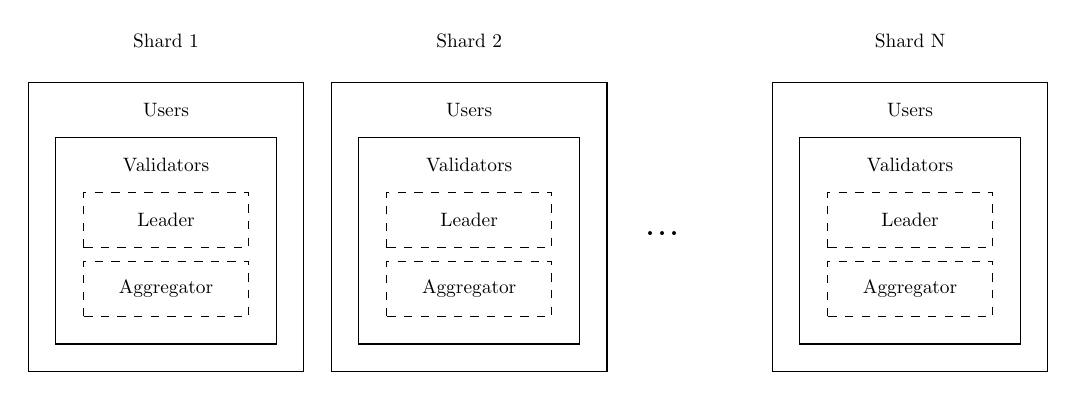
\begin{tikzpicture}[scale=0.7, every node/.style={transform shape}]
  
  %\draw[step=1cm,gray,very thin] (0,0) grid (20,7);
  
  % ***************** SHARD 1 ***************** 
  \node at (2.5,6) {Shard 1};
  
  \draw (0,0) rectangle (5,5.25);
  \node at (2.5,4.75) {Users};
  
  \draw (0.5,0.5) rectangle (4.5,4.25);
  \node at (2.5,3.75) {Validators};
  
  \draw[dashed] (1,2.25) rectangle (4,3.25);
  \node at (2.5,2.75) {Leader};
  
  \draw[dashed] (1,1) rectangle (4,2);
  \node at (2.5,1.5) {Aggregator};
  
  % ***************** SHARD 2 ***************** 
  \node at (8,6) {Shard 2};
  
  \draw (5.5,0) rectangle (10.5,5.25);
  \node at (8,4.75) {Users};
  
  \draw (6,0.5) rectangle (10,4.25);
  \node at (8,3.75) {Validators};
  
  \draw[dashed] (6.5,2.25) rectangle (9.5,3.25);
  \node at (8,2.75) {Leader};
  
  \draw[dashed] (6.5,1) rectangle (9.5,2);
  \node at (8,1.5) {Aggregator};
  
  % ***************** DOTS ***************** 
  
  \node at (11.5,2.5) {\Huge{...}};
  
  % ***************** SHARD N ***************** 
  \node at (16,6) {Shard N};
  
  \draw (13.5,0) rectangle (18.5,5.25);
  \node at (16,4.75) {Users};
  
  \draw (14,0.5) rectangle (18,4.25);
  \node at (16,3.75) {Validators};
  
  \draw[dashed] (14.5,2.25) rectangle (17.5,3.25);
  \node at (16,2.75) {Leader};
  
  \draw[dashed] (14.5,1) rectangle (17.5,2);
  \node at (16,1.5) {Aggregator};
  
  \end{tikzpicture}
  \caption{An overview of entities in the Bazo blockchain.\label{fig:Entities}}
\end{figure}

Figure \ref{fig:Entities} shows that entities are equally partitioned into shards $1$ to $N$. While users and validators always remain in their particular shard based on their wallet address $pk_{wall}$, leaders and aggregators change block-wise. An aggregator is randomly elected in-shard and a validator is randomly elected cross-shard.

Furthermore, when a user wants to join the set of validators it must create an additional public-private key-pair using RSA and publish a stake transaction containing the public key. Note that this key-pair differs to the key-pair used to sign transactions. In the rest of this paper, we refer to this RSA key-pair as to the user's \textit{commitment keys} $(pk_{comm}, sk_{comm})$.

\subsection{Network Sharding}
\label{Design:NetworkSharding}

The Bazo infrastructure is divided into several subgroups referred to as \textit{shard}, each having it's own blockchain called \textit{shardchain}. Transactions of users are stored in a transaction pool by every validator in the network, but are only validated by validators based on the public wallet address $pk_{wall}$ of sender or receiver. For example, a validator $V$ of shard $S$ is responsible for user $U$ and validates transactions where $U$ is either sender or receiver of funds in a transaction. Thus, user $U$ is \textit{assigned} to shard $S$.

Likewise, validators are only responsible for the maintenance of the shardchain based on their $pk_{wall}$. Maintenance is hereby defined as validating blocks and storing the full shardchain. Responsibilities of leaders are outlined in Section \ref{Design:TransactionSharding}. 

Note that users also receive blocks but unlike validators, they do not participate in the validation process, which is further explained in Section \ref{Design:TransactionValidation}. Users in Bazo can be compared to SPV clients in Bitcoin, i.e., they only store their own transactions and block headers of the shardchain they belong to. To put it differently, validators store every block header received from the network, but only validate blocks based on their $pk_{wall}$.

\subsection{Epochs} 

The algorithm proceeds in \textit{epochs}. An epoch $e$ ends after a predefined number of blocks, that is, assume that epoch length $length_{ep} = 100$. Epoch $e$ starts at block number $1$ and ends after block number $100$, and the next epoch $e + 1$ starts at block number $101$ and ends after block number $200$, and so on. Furthermore, the process of ending an epoch is called \textit{finalization}. An epoch finalizes with a special type of block called \textit{epoch block}, denoted $eb$. An epoch block serves as a marker. Epoch finality is further explained in Section \ref{Design:Finality}.

\begin{figure}[hbt]
\centering
\captionsetup{justification=centering}
  \begin{tikzpicture}[scale=0.9, every node/.style={transform shape}]
      % Setup the style for the states
      \tikzset{node style/.style={state,minimum width=8mm,minimum height=8mm,rectangle}}
  
      \node[node style]                (eb1) {$eb^1$};
      
      \node[node style, right=of eb1] (sb22) {$sb_2^2$};
      \node[node style, above=of sb22] (sb12) {$sb_1^2$};
      \node[node style, below=of sb22] (sb32) {$sb_3^2$};
      
      \node[node style, right=of sb22] (sb23) {$sb_2^3$};
      \node[node style, above=of sb23] (sb13) {$sb_1^3$};
      \node[node style, below=of sb23] (sb33) {$sb_3^3$};
      
      \node[node style, right=of sb23] (sb24) {$sb_2^4$};
      \node[node style, above=of sb24] (sb14) {$sb_1^4$};
      \node[node style, below=of sb24] (sb34) {$sb_3^4$};
      
      \node[node style, right=of sb24] (eb5)   {$eb^5$};
      
      \node[node style, right=of eb5] (sb26) {$sb_2^6$};
      \node[node style, above=of sb26] (sb16) {$sb_1^6$};
      \node[node style, below=of sb26] (sb36) {$sb_3^6$};
      
      \node[draw=none,  right=of sb26]   (sb2dots) {$\cdots$};
      \node[draw=none,  right=of sb16]   (sb1dots) {$\cdots$};
      \node[draw=none,  right=of sb36]   (sb3dots) {$\cdots$};
  
  \draw[>=latex,
        auto=left,
        every loop]
       (sb12)   edge node {}   (eb1)
       (sb22)   edge node {}   (eb1)
       (sb32)   edge node {}   (eb1)
       
       (sb13)   edge node {}   (sb12)
       (sb23)   edge node {}   (sb22)
       (sb33)   edge node {}   (sb32)
       
       (sb14)   edge node {}   (sb13)
       (sb24)   edge node {}   (sb23)
       (sb34)   edge node {}   (sb33)
       
       (eb5)   edge node {}   (sb14)
       (eb5)   edge node {}   (sb24)
       (eb5)   edge node {}   (sb34)
       
       (sb16)   edge node {}   (eb5)
       (sb26)   edge node {}   (eb5)
       (sb36)   edge node {}   (eb5)
       
       (sb1dots)   edge node {}   (sb16)
       (sb2dots)   edge node {}   (sb26)
       (sb3dots)   edge node {}   (sb36); 
       
  \end{tikzpicture}
  \caption{The concept of epochs with number of shards $NofShards = 3$ and epoch length $length_{ep} = 3$.}
  \label{fig:shard_overview}
\end{figure}

An example is shown in Figure \ref{fig:shard_overview}. The Bazo blockchain starts with epoch block $eb^{h}$ and partitions the state into three shardchains $sb_{1-3}^h$, where $sb_{1-3}$ is a shard block of shardchain between one and three, and where $h$ is the block height. In this example, epoch length $length_{ep} = 3$. Thus, if three blocks have been created since the last epoch block, the current epoch is being finalized. Epoch block $eb^5$ is non-interactively created.

\subsection{Number of Shards}
\label{Design:NumberOfShards}

The number of shards is an important property that determines the overall scalability of the blockchain. As the number of transaction increases, the computational resources and network bandwidth required for processing transactions increases for each individual node. A balance between the number of users and the number of shards is crucial because
\begin{enumerate}
  \item having only one shard is equal to a blockchain without sharding, 
  \item having too few shards only scales sub-linearly as the number of users increases, or
  \item having too many shards increases the communication overhead required to synchronize the block height.
\end{enumerate}
Hence, a load-balancing algorithm is required to dynamically adjust the number of shards as new users are joining and using the network. 

As a first approach, the number of shards could be determined by the sum of all staked coins of the network divided by a predefined constant value that specifies the staking power per shard. This approach has the advantage that the number of shards increases (or decreases) in proportion to the actual staking power of the network. Unfortunately, the number of shards could easily be faked by a single user with a large amount of staked coins. 

A second approach would be to determine the number of shards by dividing the number of all validators of the network by a predefined constant value that specifies the number of validators per shard. This approach has the advantage that the number of shards increases (or decreases) in proportion to the actual number of validators of the network. However, the disadvantage of this approach is that the number of shards can easily be faked by a user with many wallets containing a few coins.

The last approach is to determine the number of shards by the Equation
\begin{gather}
\label{eq:NofShards}
  NofShards = \left\lceil \frac{NofUsers}{NofUsersPerShard} \right\rceil,
\end{gather}
where \textit{NofUsers} is the total amount users of the network, and where \textit{NofUsersPerShard} is a predefined value that specifies the number of users per shard. The second step is to verify if the number of shards is lower than the number of validators, i.e., 
\begin{gather}
\label{eq:NofShardsVerify}
  NofShards \geq NofValidators,
\end{gather}
where \textit{NofValidators} is the total amount of validators of the network. If \textit{NofValidators} is lower than \textit{NofShards}, Equation \ref{eq:NofShards} is recalculated with a lower \textit{NofUsersPerShard} until Equation \ref{eq:NofShardsVerify} is true. 

While the number of validators is known to each validator, it is important to point out that the total amount of all users is not known and cannot be easily calculated since every shard maintains a different amount of users. Instead, the number of users a shard maintains is contained in the header of every shard block $sb$, and a validator derives the number of users \textit{NofUsers} by adding up the \textit{NofUsersInShard} property of each block, that is, 
\begin{gather}
  NofUsers = \Sigma^{NofShards}_{i = 1} UsersInShard(sb^{h}_{i}),
\end{gather}
where $h$ is the block height, where $1 \leq i \leq NofShards$ is the shard identifier, where \textit{UsersInShard} is a function that returns the value of the number of users in shard $i$ of a block. Note that validators only store blocks of their assigned shard until an epoch ends because the increase or decrease of the number of shards is unknown ahead of the next epoch resulting in a more or less partitioning of the network. For example, a validator can be responsible for blocks of shard 2 (of 3 in total) in epoch $e$ and responsible for blocks of shard 3 (of 4 in total) in epoch $e + 1$.
\begin{figure}[hbt]
  \centering
  \begin{tikzpicture}
    \tikzset{node style/.style={state,node distance=7mm,minimum width=3mm,minimum height=3mm,rectangle}}
  
    \node[node style]                             (ebx0) {};
    \node[node style, right=of ebx0]              (sb21) {};
    \node[node style, above=of sb21]              (sb11) {};
    \node[node style, below=of sb21]              (sb31) {};
    \node[node style, right=of sb21]              (sb22) {};
    \node[node style, above=of sb22]              (sb12) {};
    \node[node style, below=of sb22]              (sb32) {};
    \node[node style, right=of sb32]              (sb33) {};
    \node[node style, right=of sb22]              (sb23) {};
    \node[node style, right=of sb12]              (sb13) {};
    \node[node style, right=of sb23]              (ebx4) {};
    \node[node style, above right=0.7cm of ebx4] (sb25) {};
    \node[node style, above=of sb25]              (sb15) {};
    \node[node style, below right=0.7cm of ebx4] (sb35) {};
    \node[node style, below=of sb35]              (sb45) {};
    \node[node style, right=of sb15]              (sb16) {};
    \node[node style, right=of sb16]              (sb17) {};
    \node[node style, right=of sb25]              (sb26) {};
    \node[node style, right=of sb26]              (sb27) {};
    \node[node style, right=of sb35]              (sb36) {};
    \node[node style, right=of sb36]              (sb37) {};
    \node[node style, right=of sb45]              (sb46) {};
    \node[node style, right=of sb46]              (sb47) {};
    \node[node style, right=3.7cm of ebx4]        (ebx8) {};
    \node[node style, above right=0.7cm of ebx8]  (sb19) {};
    \node[node style, below right=0.7cm of ebx8]  (sb29) {};
    \node[node style, right=of sb19]              (sb110) {};
    \node[node style, right=of sb29]              (sb210) {};
    \node[draw=none, right=of sb110]              (sb111) {};
    \node[draw=none, right=of sb210]              (sb211) {};
  
  \draw[>=latex,
      auto=left,
      every loop]
     (sb11) edge node {} (ebx0)
     (sb21) edge node {} (ebx0)
     (sb31) edge node {} (ebx0)
     (sb12) edge node {} (sb11)
     (sb22) edge node {} (sb21)
     (sb32) edge node {} (sb31)
     (sb13) edge node {} (sb12)
     (sb23) edge node {} (sb22)
     (sb33) edge node {} (sb32)
     (sb15) edge node {} (ebx4)
     (sb25) edge node {} (ebx4)
     (sb35) edge node {} (ebx4)
     (sb45) edge node {} (ebx4)
     (ebx4) edge node {} (sb13)
     (ebx4) edge node {} (sb23)
     (ebx4) edge node {} (sb33)
     (sb16) edge node {} (sb15)
     (sb17) edge node {} (sb16)
     (sb26) edge node {} (sb25)
     (sb27) edge node {} (sb26)
     (sb36) edge node {} (sb35)
     (sb37) edge node {} (sb36)
     (sb46) edge node {} (sb45)
     (sb47) edge node {} (sb46)
     (ebx8) edge node {} (sb17)
     (ebx8) edge node {} (sb27)
     (ebx8) edge node {} (sb37)
     (ebx8) edge node {} (sb47)
     (sb19) edge node {} (ebx8)
     (sb29) edge node {} (ebx8)
     (sb110) edge node {} (sb19)
     (sb210) edge node {} (sb29);
     
  \draw[dashed] 
     (sb111) edge node {} (sb110)
     (sb211) edge node {} (sb210);
  
  \end{tikzpicture}
  \caption{Load-balancing dynamically adjusts the number of shards to maximize throughput and minimize overload of a single node.}
\end{figure}

\section{Identity Setup and Leader Formation}

Validators are users that have joined the set of validators by publishing a StakeTx containing the public commitment key $pk_{comm}$ to the network, which is explained in more detail in \cite{Blum18}. However, and in order for validators to get the right to append a block to a shardchain, they have to be elected as a leader and assigned to a shard.

\subsection{Leader Election}
\label{Design:LeaderElection}

The leader election process is identical to the process of fulfilling PoS condition introduced in \cite{Bachmann18}, which was further revised in \cite{Blum18} due to a security vulnerability. 

Each validator participates in the leader election process in a non-interactive way. Contrary to PoW, a validator is limited to exactly 1 H/s (hash per second) by providing a valid \textit{TimeInSeconds} to fulfill the PoS condition  

\begin{gather}
\label{eq:PoSCondition}
  {\frac{\text{SHA3-512}([Proof_{PrevBlocks}] \cdot Proof_{Local} \cdot Role \cdot TimeInSeconds)}{Coins}} \leq Target,
\end{gather}
% TODO in implementation: Change SHA-256 to SHA3-512
\noindent where

\begin{gather}
  Proof_{Local} = RSA(sk_{comm}, \text{SHA3-512}(BlockHeight)).
\end{gather}

\noindent
The PoS condition consists of the following properties:

\begin{description}
  \item[List of the Previous Proofs ($Proof_{PrevBlocks}$)] By including a list of the previous proofs of a particular shard, a stake grinding attack becomes infeasible.
  \item[Local Proof ($Proof_{Local}$)] All parameters are the same for each validator in the network except the local proof. The local proof individualizes the PoS condition to each validator and therefore, a validator with a low amount of coins also has the possibility to append a block to the blockchain.
  \item[Election Role($Role$)] Determines the role for which a validator wants to be elected for. This property is set to $"L"$ for the leader election process and set to $"A"$ for the aggregator election process.
  \item[Amount of Coins($Coins$)] The amount of coins a leader owns. Note that the chances increase proportionally to the number of $Coins$.
  \item[Difficulty of the PoS condition($Target$)] A validator has to fall below a \textit{Target} in order to append the next block to the blockchain. Note that this target determines the speed of the blockchain. As the number of validators in-/decreases the difficulty must be adjusted accordingly.
\end{description}

If a validator falls below the $Target$ value, he or she becomes a leader. A leader has the right to append the next block to a particular shardchain. The system detects malicious attackers who attempt to speed up his hashing power, e.g. by manipulating the clock speed. The probability of a validator being elected to append the next block is in proportion to the stake he or she has. For example, a validator with 50 coins has a 5 times higher chance than a validator with 10 coins. The parameters in Equation \ref{eq:PoSCondition} correspond to a validator's $pk_{wall}$, i.e., the validator uses the proofs $[Proof_{PrevBlocks}]$ and the block height $BlockHeight$ of the shardchain they are assigned to.

\subsection{Leader Assignment}
\label{Design:LeaderAssignment}

Permitting a leader to choose the shard he or she wants to append a block is insecure. Thus, we need a way to introduce randomness to securely assign a leader to a shard. True randomness is crucial to achieve a fair election among stakeholders, otherwise the algorithm may be prone to manipulation by an adversary \parencite{Ouroboros2016}. Thus, we decided to assign a leader to a shard in a non-interactive way using only information that is locally available to each validator. A leader is assigned to a shard using parts of the PoS condition \ref{eq:PoSCondition}, that is, 

\begin{gather}
\label{eq:LeaderAssignment}
  \text{SHA3-512}([Proof_{PrevBlocks}] \cdot Proof_{Local} \cdot Role \cdot TimeInSeconds)\ mod\ NofShards,
\end{gather}

\noindent Notice that part of Equation \ref{eq:LeaderAssignment} is just the dividend of the fraction of Equation \ref{eq:PoSCondition}, and thus, the description of properties are identical, except the property \textit{NofShards}.

\begin{description}
  \item[Number of Shards ($NofShards$)] A leader is assigned to a shard by using the remainder of the modulo operation with the number of shards the network is partitioned in to.
\end{description}

It is important to realise that this mechanism cannot ensure that every shard has a leader for a specific block height. At block height $h$, a shard can have zero or more (up to the number of validators) leaders. In the case that two or more leaders are assigned to the same shard, the leader with the lowest \textit{Target} has the right to create the next block. 

\subsection{New Validators Joining Bazo}

Users can express their intention to join the set of validators by sending a StakeTx to the network at any time. Since users only store block headers of the shard they are assigned to, a bootstrapping process to download the shardchains history would be required. The bootstrap time includes the time to download the block headers of a shard and the time to process the history necessary to validate the current system state. Hence, and for the sake of simplicity, new validators do not immediately join the set of validators and instead have to wait until the current epoch ends before they can participate in the leader election process.

\section{Transaction Sharding and Processing}
\label{Design:TransactionSharding}

In Section \ref{Design:NetworkSharding}, we presented a way on how to partition the network into shards, with each shard capable of parallelized transaction processing. In this Section, we present how transactions are assigned to shards.

\subsection{Self-Contained Proofs}
\label{Design:SelfContainedProofs}

The core of Bazo's consensus protocol relies on \textit{self-contained proofs} (SCPs), a new primitive for blockchain protocols to prove that a user has sufficient funds without relying on the blockchain history at all.
% TODO: Write this better! 
Instead of validators requiring the full blockchain to validate a transaction, a user has to provide all required proofs in the transaction in order for validators to verify a transaction, independent of the blockchain.
 
A self-contained proof consists of Merkle proofs provided by the sender of a transaction. A sender has to provide one Merkle proof for each transaction sent since the last epoch. % TODO in implementation: is one epoch of the past sufficient (security)?
Validators could know the number of proofs a sender has to provide by comparing the current transaction counter of an account with the transaction counter of the last epoch. However, performing checks against the transaction counter is not sufficient and further checks must be performed, elaborated in Section \ref{Design:BlockHeightSync} and reasoned in Section \ref{Eval:AttackScenarios}.

\begin{example}
\label{ex:SCPExample}
Consider a shardchain as shown in Figure \ref{fig:SCPExample}. Assume that user $A$ is also a validator and hence has the complete history of the shardchain since the last epoch. Further assume that user $A$ has already transmitted two funds transactions $F3$ and $F6$. User $A$ wants to create a new transaction and send it to the network. Therefore, a self-contained proof must contain two Merkle proofs, one for each transaction $F3$ and $F6$, i.e., $SCP = \{Proof_1, Proof_2\}$, where $Proof_1 = \{F5, F6, B2\}$ and $Proof_2 = \{F3, F4, A1\}$. Note that a SCP contains a Merkle proof for the most recent transaction first.

\begin{figure}[hbt]
\centering
\begin{tikzpicture}[scale=0.65,node distance=20mm, 
  every node/.style={transform shape},
  level/.style={sibling distance=40mm/#1}
]

\tikzstyle{vertex}=[draw,circle,minimum size=36pt,inner sep=0pt]
\tikzstyle{vertexsmall}=[draw,circle,minimum size=24pt,inner sep=0pt]
\tikzset{node style/.style={state,minimum width=12mm,minimum height=12mm,rectangle}}

\node[node style]              (b1){};
\node[node style, right=of b1] (b2){};
\node[node style, right=of b2] (b3){};
\node[node style, right=of b3] (b4){};
\node[node style, right=of b4] (b5){};
\node[node style, right=of b5] (b6){};

\node [vertex,below=1cm of b2] (r1){$M1$}
  child {
    node [vertex] {$A1$}
    child {
      node [vertex] {$F1$}
    }
    child {
      node [vertex] {$F2$}
    }
  }
  child {
    node [vertex] {$A2$}
    child {
      node [vertex,very thick] {$F3$}
    }
    child {
      node [vertex] {$F4$}
    }
  };


\node [vertex,below=1cm of b5] (r2){$M2$}
  child {
    node [vertex] {$B1$}
    child {
      node [vertex] {$F5$}
    }
    child {
      node [vertex,very thick] {$F6$}
    }
  }
  child {
    node [vertex] {$B2$}
    child {
      node [vertex] {$F7$}
    }
    child {
      node [vertex] {$F8$}
    }
  };
  
\draw[>=latex,auto=left,every loop]
  (b2) edge node {} (b1)
  (b3) edge node {} (b2)
  (b4) edge node {} (b3)
  (b5) edge node {} (b4)
  (b6) edge node {} (b5); 
 
\draw[thin,shorten >=4pt,shorten <=4pt,>=stealth,dotted]
  (r1) edge node {}   (b2)
  (r2) edge node {}   (b5);
   
\end{tikzpicture}   
\caption{Initial situation of an SCP example: A user has to include two Merkle proofs for $F3$ and $F6$ in the next transaction.\label{fig:SCPExample}}
\end{figure}  
This example also applies for transactions where user $A$ received funds or aggregated transactions. In fact, performing block-wise transaction aggregation by sender performed by the leader creating a block helps mitigating fraudulent proofs, as evaluated in Section \ref{Eval:AttackScenarios}.
\end{example}

From example \ref{ex:SCPExample} we can also conclude a maximum size of a self-contained proof. Assuming that $length_{ep}$ is the epoch length and a shard block can contain up to $m$ transaction of size $s$, we derive the upper bound of a self-contained proof being equal to
\begin{gather}
  length_{ep} \cdot log(m) \cdot s = \mathcal{O}(length_{ep}).
\end{gather}

\subsection{Transaction Validation}
\label{Design:TransactionValidation}

Once leaders have been assigned to a shard, each leader has to create a new block with transactions based on the assigned shard and the transaction. Each transaction consists of a \textit{self-contained proof} that refers back to the final state of the last epoch. With self-contained proofs, validators are able to verify transactions without relying on external resources, i.e., only the final state of the last epoch and the self-contained proof contained in a transaction is required for verification. 

Each validator locally maintains a transaction pool with all transactions of the network, and when a validator becomes a leader of shard, the following steps are taken by the leader at block height $h$ to create block $b$:

\begin{enumerate}
  \item The leader picks transactions from the local transaction pool with
    \begin{gather}
    \label{eq:NetworkSharding}
      s = pk_{wall}\ mod\ NofShards,
    \end{gather}
    where $s$ is the assigned shard, where $pk_{wall}$ is the wallet address of the sender or receiver, where $mod$ denotes the mathematical modulo operation, and where \textit{NofShards} refers to the number of shards the network is partitioned in to.
  \item For each transaction, the leader verifies the signature of the transaction using the public key $pk_{wall}$ of the transaction sender $tx_{send}$. If the signature is valid, continue. Otherwise, the transaction contains no valid signature and the algorithm stops.
  \item The leader then proceeds to check the self-contained proof containing one or more Merkle proofs. Using the block headers of shard $s$, the leader performs the following subtask, iteratively going back starting with block $sb_s^{x}$, where $x \leftarrow h - 1$:
    \begin{enumerate}
      \item By querying the Bloom filter, the leader can check if $sb_s^{x}$ contains a transaction of $tx_{send}$. If yes, continue. Otherwise the block contains no transaction of $tx_{send}$, set $x \leftarrow x - 1$ and repeat step.
      \item Generate Merkle root $r$ by using the Merkle proof provided in the self-contained proof. If $r = MerkleRoot(sb_s^{x})$, where \textit{MerkleRoot} is a function which returns the Merkle root of a block, set $x \leftarrow x - 1$ and repeat subtask for each Merkle proof until all proofs are checked. Otherwise, the self-contained proof is missing a Merkle proof not provided by $tx_{send}$ and thus, the transaction is invalid and discarded. Section \ref{Eval:AttackScenarios} elaborates on the necessity of this subtask.
    \end{enumerate} 
  \item Once a block is full, i.e., the maximum amount of transactions that fit into a block is reached, the leader adds a staking proof to the block. The staking proof proves that the leader has sufficient funds and that he or she fulfills the minimum staking amount requirement. The staking proof is also a self-contained proof containing one or more Merkle proofs. 
  \item Lastly, the leader follows the standard block creation procedure, which includes generating the Merkle root, creating the Bloom filter, hashing the block, etc.
\end{enumerate}

Once this process is finished, the block is sent to the network for distribution.

Upon receiving block $b$, validators of shard $s$ query for all transactions that are contained within the block and verify the validity. If $b$ is valid, the block is appended to the chain of shard $s$. Otherwise, the leader who proposed block $b$ gets slashed and validators wait for another block for block height $h$.

Note that Bloom filters have a false-positive rate of 10\% in our system. A user constructing a self-contained proof has to provide an additional proof for each invalid return value of the Bloom filter, i.e., the user has to prove that a transaction is \textit{not} in the block that returns a false-positive. Since transactions (leaves) in a Merkle tree are in ascending order, a user only has to provide a Merkle proof that shows that the transaction in question is not part of the Merkle tree. Example \ref{ex:BloomFalsePositive} conceptually describes a possible scenario.

\begin{example}
\label{ex:BloomFalsePositive}
Consider a block containing transactions $\{0x12, 0x15, 0x17, 0x18\}$. The Bloom filter of the block returns a false-positive for transaction $0x14$. Figure \ref{fig:BloomFalsePositive} shows the Merkle tree of the block with the leaves in in ascending order. In that case, a user has to provide a Merkle proof that contains $\{0x12, 0x15, H2\}$ deeming the false-positive invalid.
\begin{figure}[hbt]
\centering
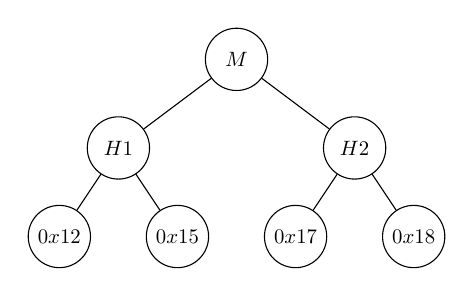
\begin{tikzpicture}[scale=0.75,node distance=20mm, 
  every node/.style={transform shape},
  level/.style={sibling distance=40mm/#1}
]

\tikzstyle{vertex}=[draw,circle,minimum size=30pt,inner sep=0pt]

\node [vertex] (r1){$M$}
  child {
    node [vertex] {$H1$}
    child {
      node [vertex] {$0x12$}
    }
    child {
      node [vertex] {$0x15$}
    }
  }
  child {
    node [vertex] {$H2$}
    child {
      node [vertex] {$0x17$}
    }
    child {
      node [vertex] {$0x18$}
    }
  };
\end{tikzpicture}  
\caption{Transactions in Merkle trees are in ascending order\label{fig:BloomFalsePositive}}
\end{figure}  
\end{example}

\subsection{Transaction Aggregation}
\label{Design:TransactionAggregation}

Transaction aggregation is a way of keeping the size of the ledger small, that is, validators only store transactions not older than a predefined number of blocks, denoted as aggregation length $length_{ag}$. A special type of transaction called \textit{Aggregation Transaction (AggTx)} is created by summing up transferred amounts either by sender or by receiver.

\begin{figure}[hbt]
\centering
\begin{subfigure}[b]{0.9\textwidth}
  \centering
  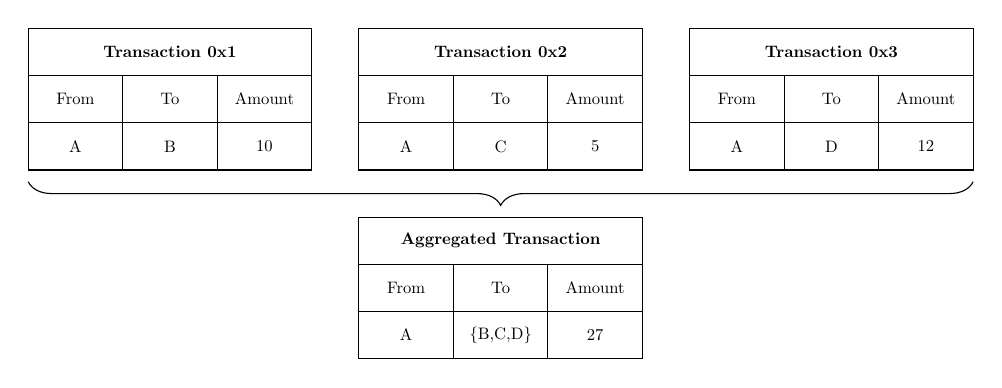
\begin{tikzpicture}[scale=0.6, every node/.style={transform shape}]

  % ***************** Agg Tx ***************** 
  
  \draw (7,0) rectangle (13,3);
  \draw (7,2) -- (13,2);
  \draw (9,0) -- (9,2);
  \draw (11,0) -- (11,2);
  \draw (7,1) -- (13,1);
  
  \node at (10,2.5) {\bfseries{Aggregated Transaction}};
  \node at (8,1.5) {From};
  \node at (8,0.5) {A};
  \node at (10,1.5) {To};
  \node at (10,0.5) {\{B,C,D\}};
  \node at (12,1.5) {Amount};
  \node at (12,0.5) {27};
  
  % ***************** TX 1 ***************** 
  
  \draw (0,4) rectangle (6,7);
  \draw (0,6) -- (6,6);
  \draw (2,4) -- (2,6);
  \draw (4,4) -- (4,6);
  \draw (0,5) -- (6,5);
  
  \node at (3,6.5) {\bfseries{Transaction 0x1}};
  \node at (1,5.5) {From};
  \node at (1,4.5) {A};
  \node at (3,5.5) {To};
  \node at (3,4.5) {B};
  \node at (5,5.5) {Amount};
  \node at (5,4.5) {10};
  
  % ***************** TX 2 ***************** 
  
  \draw (7,4) rectangle (13,7);
  \draw (7,6) -- (13,6);
  \draw (9,4) -- (9,6);
  \draw (11,4) -- (11,6);
  \draw (7,5) -- (13,5);
  
  \node at (10,6.5) {\bfseries{Transaction 0x2}};
  \node at (8,5.5) {From};
  \node at (8,4.5) {A};
  \node at (10,5.5) {To};
  \node at (10,4.5) {C};
  \node at (12,5.5) {Amount};
  \node at (12,4.5) {5};
  
  % ***************** TX 2 ***************** 
  
  \draw (14,4) rectangle (20,7);
  \draw (14,6) -- (20,6);
  \draw (16,4) -- (16,6);
  \draw (18,4) -- (18,6);
  \draw (14,5) -- (20,5);
  
  \node at (17,6.5) {\bfseries{Transaction 0x3}};
  \node at (15,5.5) {From};
  \node at (15,4.5) {A};
  \node at (17,5.5) {To};
  \node at (17,4.5) {D};
  \node at (19,5.5) {Amount};
  \node at (19,4.5) {12};
  
  % ***************** BRACE ***************** 
  
  \draw[decoration={brace,mirror,amplitude=3mm},decorate]
    (0,3.75) -- node[right=12pt] {} (20,3.75);
  
  \end{tikzpicture}
  \caption{Transaction aggregation by sender.\label{fig:TxAggBySender}}
\end{subfigure}
\par\bigskip
\begin{subfigure}[b]{0.9\textwidth}
  \centering
  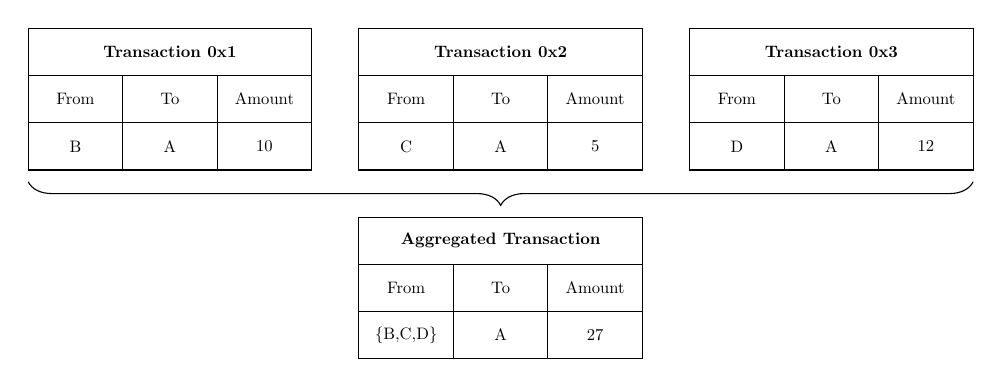
\begin{tikzpicture}[scale=0.6, every node/.style={transform shape}]
  % ***************** Agg Tx ***************** 
  
  \draw (7,0) rectangle (13,3);
  \draw (7,2) -- (13,2);
  \draw (9,0) -- (9,2);
  \draw (11,0) -- (11,2);
  \draw (7,1) -- (13,1);
  
  \node at (10,2.5) {\bfseries{Aggregated Transaction}};
  \node at (8,1.5) {From};
  \node at (8,0.5) {\{B,C,D\}};
  \node at (10,1.5) {To};
  \node at (10,0.5) {A};
  \node at (12,1.5) {Amount};
  \node at (12,0.5) {27};
  
  % ***************** TX 1 ***************** 
  
  \draw (0,4) rectangle (6,7);
  \draw (0,6) -- (6,6);
  \draw (2,4) -- (2,6);
  \draw (4,4) -- (4,6);
  \draw (0,5) -- (6,5);
  
  \node at (3,6.5) {\bfseries{Transaction 0x1}};
  \node at (1,5.5) {From};
  \node at (1,4.5) {B};
  \node at (3,5.5) {To};
  \node at (3,4.5) {A};
  \node at (5,5.5) {Amount};
  \node at (5,4.5) {10};
  
  % ***************** TX 2 ***************** 
  
  \draw (7,4) rectangle (13,7);
  \draw (7,6) -- (13,6);
  \draw (9,4) -- (9,6);
  \draw (11,4) -- (11,6);
  \draw (7,5) -- (13,5);
  
  \node at (10,6.5) {\bfseries{Transaction 0x2}};
  \node at (8,5.5) {From};
  \node at (8,4.5) {C};
  \node at (10,5.5) {To};
  \node at (10,4.5) {A};
  \node at (12,5.5) {Amount};
  \node at (12,4.5) {5};
  
  % ***************** TX 2 ***************** 
  
  \draw (14,4) rectangle (20,7);
  \draw (14,6) -- (20,6);
  \draw (16,4) -- (16,6);
  \draw (18,4) -- (18,6);
  \draw (14,5) -- (20,5);
  
  \node at (17,6.5) {\bfseries{Transaction 0x3}};
  \node at (15,5.5) {From};
  \node at (15,4.5) {D};
  \node at (17,5.5) {To};
  \node at (17,4.5) {A};
  \node at (19,5.5) {Amount};
  \node at (19,4.5) {12};
  
  % ***************** BRACE ***************** 
  
  \draw[decoration={brace,mirror,amplitude=3mm},decorate]
    (0,3.75) -- node[right=12pt] {} (20,3.75);
  
  \end{tikzpicture}
  \caption{Transaction aggregation by receiver.\label{fig:TxAggByReceiver}}
\end{subfigure}
\caption{Transaction aggregation types}
\end{figure}

In transaction aggregation by sender, transactions sent \textit{from} a particular user are summed up, shown in Figure \ref{fig:TxAggBySender}. On the contrary, in transaction aggregation by receiver, transactions sent \textit{to} a particular user are summed up, shown in Figure \ref{fig:TxAggByReceiver}. Furthermore, we distinguish between transaction aggregation performed by an aggregator or by a leader.

Firstly, transaction aggregation is performed by validators with the role \textit{aggregator}. An aggregator is elected per block height and per shard in the same way a leader is elected with the exception that the \textit{Role} property of Equation \ref{eq:PoSCondition} must be set to $"A"$. In rare cases, there can be zero or more aggregators per block height. If more than one validator fulfills the PoS condition \ref{eq:PoSCondition}, the validator who has the lowest value below \textit{Target} becomes an aggregator. Also note that an elected aggregator is not assigned to a random shard. An aggregator only aggregates transactions of the shard they are assigned to, because block bodies containing transactions with self-contained proofs are only stored by validators of the shard they are assigned.

After becoming an aggregator, transactions from previous blocks are aggregated by sender or receiver. Aggregated transactions are then filled into a special type of block called \textit{aggregation block}. An aggregation block of shard $s$ at block height $h$ serves as a proposal to a validator who becomes a leader of shard $s$ at block height $h + 1$. Informally, the following algorithm is performed by each aggregator at block height $h$:
\begin{enumerate}
  \item Create an empty aggregation block.
  \item Pick transactions in two ways:
    \begin{enumerate}
      \item For each shard block or aggregation block $b$, where $Height(b) \leq h - 1$, pick  transactions where each sender or receiver appears at least twice and where $Aggregated = false$. Note that $FundsTx$ as well as $AggTx$ can be aggregated.
      \item For each shard or aggregation block $b$, where $h - Height(b) \geq length_{ag}$, pick all transactions which have not been aggregated yet, i.e., where $Aggregated = false$.
    \end{enumerate}
  \item Sum up the amount of coins that have been sent or received, generate the transaction hash, create the aggregated transaction and add it to the aggregation block. Set $Aggregated \leftarrow true$ to transactions in the block they were picked from.
\end{enumerate}

Secondly, transaction aggregation is performed by validators with the role \textit{leader}. When a leader creating a block picks transaction from the local transaction pool, transactions of the same sender are aggregated to a single aggregated transaction. This task is crucial in order to prevent fraudulent proofs, evaluated in Section \ref{Eval:SecurityConsiderations}. A leader is also responsible for the verification at height $h$ of an aggregation block that has been proposed at block height $h - 1$. The verification process is performed in the same fashion as Bloom filter checks of self-contained proofs.

\subsection{Block Height Synchronisation}
\label{Design:BlockHeightSync}

The leader assignment process described in Section \ref{Design:LeaderAssignment} does not guarantee to have one leader per shard. As a result, a shard could have no leader at one block height resulting in a divergence of block heights among different shardchains. For this reason, the block height of shardchains must be synchronized with each other to ensure equally growing chains of blocks.

\begin{figure}[hbt]
  \centering
  \captionsetup{justification=centering}
  \begin{subfigure}[b]{0.45\textwidth}
    \centering
    \begin{tikzpicture}
        \tikzset{node style/.style={state,node distance=7mm,minimum width=3mm,minimum height=3mm,rectangle}}
    
        \node[node style]   (sb_2-1)  {};
        \node[node style, above=of sb_2-1]  (sb_1-1)  {};
        \node[node style, below=of sb_2-1]  (sb_3-1)  {};
        \node[node style, right=of sb_2-1]  (sb_2-2) {};
        \node[node style, above=of sb_2-2]  (sb_1-2) {};
        \node[node style, below=of sb_2-2]  (sb_3-2) {};
        \node[node style, right=of sb_3-2]  (sb_3-3) {};
        \node[node style, right=of sb_3-3]  (sb_3-4) {};
        \node[node style, right=of sb_2-2] (sb_2-3)  {};
        \node[node style, right=of sb_1-2] (sb_1-3)  {};
        \node[node style, right=of sb_1-3] (sb_1-4)  {};
        \node[node style, right=of sb_1-4] (sb_1-5)  {};
    
    \draw[>=latex,
          auto=left,
          every loop]
         (sb_1-2)  edge node {}   (sb_1-1)
         (sb_2-2)  edge node {}   (sb_2-1)
         (sb_3-2)  edge node {}   (sb_3-1)
         (sb_1-3)  edge node {}   (sb_1-2)
         (sb_1-4)  edge node {}   (sb_1-3)
         (sb_1-5)  edge node {}   (sb_1-4)
         (sb_2-3) edge node {}   (sb_2-2)
         (sb_3-3) edge node {}   (sb_3-2)
         (sb_3-4) edge node {}   (sb_3-3); 
    \end{tikzpicture}
    \caption{Without Synchronisation}
  \end{subfigure}
  ~
  \begin{subfigure}[b]{0.45\textwidth}
    \centering
    \begin{tikzpicture}
        \tikzset{node style/.style={state,node distance=7mm,minimum width=3mm,minimum height=3mm,rectangle}}
    
        \node[node style]   (sb_2-1)  {};
        \node[node style, above=of sb_2-1]  (sb_1-1)  {};
        \node[node style, below=of sb_2-1]  (sb_3-1)  {};
        \node[node style, right=of sb_2-1]  (sb_2-2) {};
        \node[node style, above=of sb_2-2]  (sb_1-2) {};
        \node[node style, below=of sb_2-2]  (sb_3-2) {};
        \node[node style, right=of sb_3-2]  (sb_3-3) {};
        \node[node style, right=of sb_3-3]  (sb_3-4) {};
        \node[node style, right=of sb_2-2] (sb_2-3)  {};
        \node[node style, right=of sb_2-3] (sb_2-4)  {};
        \node[node style, right=of sb_1-2] (sb_1-3)  {};
        \node[node style, right=of sb_1-3] (sb_1-4)  {};
    
    \draw[>=latex,
          auto=left,
          every loop]
         (sb_1-2)  edge node {}   (sb_1-1)
         (sb_2-2)  edge node {}   (sb_2-1)
         (sb_3-2)  edge node {}   (sb_3-1)
         (sb_1-3)  edge node {}   (sb_1-2)
         (sb_2-3) edge node {}   (sb_2-2)
         (sb_3-3) edge node {}   (sb_3-2)
         (sb_1-4)  edge node {}   (sb_1-3)
         (sb_2-4) edge node {}   (sb_2-3)
         (sb_3-4) edge node {}   (sb_3-3); 
         
    \draw[thin,double,<->,shorten >=4pt,shorten <=4pt,>=stealth,dotted]
         (sb_1-1)   edge node {}   (sb_2-1)
         (sb_2-1)   edge node {}   (sb_3-1)
         (sb_1-2)   edge node {}   (sb_2-2)
         (sb_2-2)   edge node {}   (sb_3-2)
         (sb_1-3)   edge node {}   (sb_2-3)
         (sb_2-3)   edge node {}   (sb_3-3)
         (sb_1-4)   edge node {}   (sb_2-4)
         (sb_2-4)   edge node {}   (sb_3-4);       
         
    \end{tikzpicture}
    \caption{With Synchronisation}
  \end{subfigure}
  \caption{Shardchains could diverge during due to network latency or other reasons resulting in different block heights.}
  \label{fig:shard_divergence}
\end{figure}

Validators receive blocks and have to perform at least one comparison operation per block in order to decide whether the block belongs to their shard or not. Hence, they can keep track of the number of blocks received at block height $h$. If the number equals to \textit{NofShards}, validators can be certain that each shardchain of the network grows equally at the same pace. Informally, the following algorithm is performed by each validator $v$ upon receiving block $b$:
\begin{enumerate}
  \item The validator checks if the block has already been processed by using the hash of the block and comparing it with the local database. If the block has not been processed yet, continue. Otherwise, the block has already been processed or deemed invalid and the algorithm stops.
  \item If $Height(b) = h$, where $Height$ is a function that returns the height of block, continue. Otherwise, the block does not belong to the current block height the algorithm stops.
  \item Where \textit{ShardOfBlock} is a function that returns the shard identifier for which a block was created for, and where \textit{ShardOfValidator} is a function that returns the shard identifier the validator belongs to, 
    \begin{enumerate}
      \item if $ShardOfBlock(b) = ShardOfValidator(v)$, locally store the block header and block body. For each transaction hash included in the block, the validator queries the transaction from the local transaction pool and deletes it, otherwise,
      \item if $ShardOfBlock(b) \neq ShardOfValidator(v)$, locally store only the block header.
    \end{enumerate}
    In either case, increment $ReceivedBlocks$ by one, where $ReceivedBlocks$ keeps track of the number of received blocks for block height $h$.
  \item Check the self-contained proof. If all Merkle proofs of the SCP are valid, redistribute the block immediately. Otherwise, stop the algorithm.
  \item If $ReceivedBlocks = NofShards$, set $ReceivedBlocks \leftarrow 0$ and start the leader election process, as explained in Section \ref{Design:LeaderElection}. Otherwise, repeat algorithm on arrival of the next block.
\end{enumerate}

\section{Epoch Finality}
\label{Design:Finality}

An epoch finishes after a predefined number of blocks, called \textit{epoch length}, denoted $length_{ep}$. As pointed out in Section \ref{Design:BlockHeightSync}, shardchains can grow in a non-deterministic way if two or more leaders are assigned to the same shard, but since shardchains are synchronized among each other, the finalization of an epoch is guaranteed to end almost at the same time.

Once $length_{ep}$ is reached, validators agree on an epoch block. This special type of block only serves as checkpoint. The network is then repartitioned based on the number of users $NofUsers$. An epoch block is not distributed because it is non-interactively created by every validator in the network. Each validator is able to derive the same hash based on previous blocks.



% Chapter Implementation

\chapter{Implementation}

\label{Chapter:Implementation}

This chapter explains how the existing Bazo blockchain is revised and extended. Parts of the descriptions are taken from previous papers \cite{Sgier17, Bachmann18, Blum18} and updated where necessary.

\section{Transactions}

\subsection{Stake Transaction (StakeTx)}
\label{Impl:StakeTx}

A node wishing to participate in staking can publish a stake transaction. The transaction contains the commitment key $pk_{comm}$. The StakeTx consists of the following properties:

\begin{description}
  \item[Fee] A fee that has to be paid for the validator.
  \item[Is Staking] A boolean value that indicates whether the node wants to join or leave the set of validators.
  \item[Account] The hash of the public key of the issuer.
  \item[Key Commitment] When a node wants to join the set of validators it must create a pair of public and private keys $(pk_{comm}, sk_{comm})$ using RSA. Note that this key-pair is different to the key-pair of the user's wallet. By submitting the public key $pk_{comm}$, the node commits to this key and it cannot change it in a later step. The $(pk_{comm}, sk_{comm})$ key-pair will be used in the PoS condition \ref{eq:PoSCondition}.
  \item[Signature] The signature serves the purpose of authentication. The node digitally signs the transaction with its private key $sk_{wall}$.
\end{description}

\subsection{System Parameters (ConfigTx)}

System parameters can be adjusted with this type of transaction without the need of a hard fork. The transaction must be signed by a root account in order to be accepted. Parameters to change are for example minimum staking amount, minimum waiting time, accepted time difference, slashing window size, or slashing reward.

\subsection{Funds Transaction (FundsTx)}
\label{Impl:FundsTx}

Users can transfer funds from one account to another by using a FundsTx. In fact, transferring funds is the process of subtracting an amount of coins \textit{from} the sender's account and adding the same amount of coins \textit{to} the receiver's account.

\begin{description}
  \item[Amount] The amount of Bazo coins to be transferred between accounts.
  \item[Fee] A fee that has to be paid for the validator.
  \item[Transaction Counter] The account nonce of the sender's account, prevents replay attacks.
  \item[Aggregated] Determines whether this transaction has been aggregated or not ($true/false$).
  \item[From] The public address $pk_{wall}$ of the sender.
  \item[To] The public address $pk_{wall}$ of the receiver.
  \item[Self-contained Proof] An ordered list of Merkle proofs referring back to the last epoch block to concisely prove that the sender of the transaction has enough funds to execute the transaction.
  \item[Signature] The signature serves the purpose of authentication. The node digitally signs the transaction with its private key $sk_{wall}$.
\end{description}

\subsection{Aggregation Transaction (AggTx)}

An aggregation transaction coalesces two or more $FundsTx/AggTx$. The amount that is transferred in an aggregation transaction is the sum of all $FundsTx/AggTx$. The transaction hash of an aggregation transaction is generated with a Merkle tree whose root node represents the hash of the combined hash of its children node, and the hash of its children nodes are the hash of the combined hashes of their children nodes, and so on until the leaves, where each leaf either represents the transaction hash of a $FundsTx$ or $AggTx$. Figure \ref{fig:AggTxHash} shows the Merkle tree for generating the aggregation transaction hash\label{fig:AggTxHash}, where $F$ = $FundsTx$ hash, $H[1/2]$ = intermediate hash of two $F$s, and where $A$ = $AggTx$ hash.

\begin{figure}[hbt]
\centering
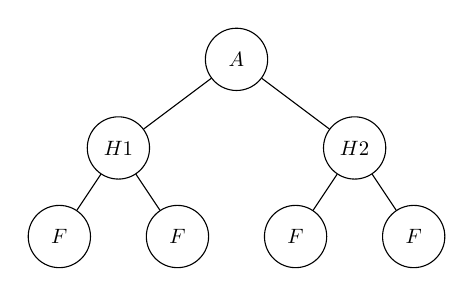
\begin{tikzpicture}[scale=0.75,node distance=20mm, 
  every node/.style={transform shape},
  level/.style={sibling distance=40mm/#1}
]

\tikzstyle{vertex}=[draw,circle,minimum size=30pt,inner sep=0pt]

\node [vertex] (r1){$A$}
  child {
    node [vertex] {$H1$}
    child {
      node [vertex] {$F$}
    }
    child {
      node [vertex] {$F$}
    }
  }
  child {
    node [vertex] {$H2$}
    child {
      node [vertex] {$F$}
    }
    child {
      node [vertex] {$F$}
    }
  };
\end{tikzpicture}  
\caption{Generating the hash of an aggregated transaction\label{fig:AggTxHash}}
\end{figure}  

\begin{description}
  \item[Hash] The transaction hash acts as a unique identifier of this aggregated transaction. The generation of the hash is shown in figure \ref{fig:AggTxHash}.
  \item[Aggregated] Determines whether this transaction has been aggregated or not ($true/false$).
  \item[Amount] The summed up value of all aggregated transaction amounts.
  \item[Transaction Counter] The value of the highest transaction counter of the aggregated transactions.
  \item[From] The public addresses $[pk_{wall}]$ of the senders.
  \item[To] The public addresses $[pk_{wall}]$ of the receivers.
  \item[Number of Transactions] The number of transactions that have been aggregated.
  \item[Hash Data FundsTxs] The hashes of all Funds Transactions (FundsTxs) included in this block in sequential order.
\end{description}

\section{Blocks}

Sharding introduces two new blocks to the system, namely epoch block and aggregation block. Multiple shardchains are running in parallel and a block of a shardchain is referred to as shard block.

Furthermore, with the introduction of transaction aggregation, validators must be able to empty blocks where all transactions have been aggregated. In that case, the pointer to the hash of a previous block would is deemed invalid. In order to keep the integrity of the blockchain, a second hash that points to the previous block without transactions is added to every block.

\begin{figure}[hbt]
\centering
\begin{subfigure}[b]{0.7\textwidth}
\centering
\begin{tikzpicture}[scale=0.8,node distance=70mm, 
  every node/.style={transform shape}
]

\tikzset{node style/.style={state,minimum width=16mm,minimum height=16mm,rectangle}}

\node[node style]              (b1){};
\node[node style, right=of b1] (b2){};

\draw[>=latex,auto=left,every loop,transform canvas={yshift=-0.25cm}]
     (b2) edge node {Previous Hash (without Tx)} (b1); 
     
\draw[>=latex,auto=left,every loop,transform canvas={yshift=0.25cm}]
     (b2) edge node {Previous Hash} (b1); 
 
\end{tikzpicture}
\caption{Before emptying a block\label{fig:DLBlockchainBefore}}
\end{subfigure}
\par\bigskip
\begin{subfigure}[b]{0.7\textwidth}
\centering
\begin{tikzpicture}[scale=0.8,node distance=70mm, 
  every node/.style={transform shape}
]

\tikzset{node style/.style={state,minimum width=16mm,minimum height=16mm,rectangle}}

\node[node style]              (b1){};
\node[node style, right=of b1] (b2){};

\draw[>=latex,auto=left,every loop,transform canvas={yshift=0cm}]
     (b2) edge node {Previous Hash (without Tx)} (b1); 
 
\end{tikzpicture}
\caption{After emptying a block\label{fig:DLBlockchainAfter}}
\end{subfigure}
\caption{Transaction aggregation results in a double-linked blockchain.}
\end{figure}

Figure \ref{fig:DLBlockchainBefore} shows two blocks where one blocks points to the previous block with two hashes. A block which only contains aggregated transactions can be emptied, resulting in an invalid previous hash. However, the second hash that points to the previous block without transactions is still valid.

\subsection{Shard Block}

A shard block is almost identical to a block introduced in Bazo before. The header of a shard block consists of the following properties:

\begin{description}
  \item[Hash] The block hash acts as a unique identifier of blocks within the blockchain.
  \item[Previous Hash] This value is equal to the identifier of the previous block in the blockchain.
  \item[Previous Hash (w/o Tx)] This value is equal to the identifier of the previous block without transactions in the blockchain. If the previous block is an epoch block, this property equals to \textbf{Previous Hash}.
  \item[Number of Bloom filter Elements] The number of elements that are in the bloom filter.
  \item[Bloomfilter] The bloom filter can be queried with $pk_{wall}$ whether the block contains a transaction of $pk_{wall}$ or not. With a false-positive rate of about 10\%, the size of the bloom filter is linearly increased or decreased to meet this target.
  \item[Number of Users In Shard] The number of users in this shard.
\end{description}

\noindent The body of a shard block consists of the following properties:

\begin{description}
  \item[Time in Seconds (Nonce)] The number of seconds that a validator needed in order to fulfill the PoS condition.
  \item[Timestamp] Refers to the block creation time (seconds elapsed since January 1, 1970 UTC).
  \item[Merkle Root] The value of the merkle tree's root node. Note that the transactions, i.e., the leaves of the Merkle tree, are ordered ascending before generating the Merkle root.
  \item[Beneficiary] The address hash of the account that receives fee payments and the block reward.
  \item[Commitment Proof] This property stores a signed message of the $Height$ that this block was created. In particular, $RSA(sk_{comm}, \text{SHA3-512}(BlockHeight))$ where $sk_{comm}$ represents the private key that corresponds to the public commitment key $pk_{comm}$ that was set in the initial StakeTx of the node. Other validators can use $pk_{comm}$ to verify the proof.
  \item[Staking Proof] The proof that the creator, i.e., the leader of this particular block is eligible to create it. This proof is similar to the self-contained proof of a FundsTx, as mentioned in Section \ref{Impl:FundsTx}.
  \item[Height] The height of a block refers to the number of previously appended blocks to the blockchain.
  \item[Shard ID] The identifier of the shard this block was created for.
  \item[Slashed Address] A validator can submit a slashing proof when appending a block, i.e., it holds the address of the misbehaving node that must be punished.
  \item[Two Conflicting Block Hashes] These two properties exhibit the block hashes where the same node has appended a block on two competing chains within the slashing window size.
  \item[Number of FundsTxs/AccTxs/ConfigTxs] Corresponds to the number of transactions of each type that are included in the block.
  \item[Hash Data FundsTxs/AccTxs/ConfigTxs] The hashes of all transactions included in this block in sequential order.
\end{description}

\subsection{Epoch Block}
\label{Impl:EpochBlock}

Opposed to shard blocks, which are created by a leader and propagated through the network to every node, epoch blocks are created non-interactively, i.e., every validator locally creates an epoch block without redistributing it based on local information. The header of an epoch block consists of the following properties:

\begin{description}
  \item[Hash] The block hash acts as a unique identifier of blocks within the blockchain.
  % \item[Previous Hash] This value is equal to the identifier of the previous block in the blockchain.
  \item[Previous Hashes] This value is equal to the identifier of the previous blocks of every shard.
  % \item[Previous Hash (w/o Tx)] This value is equal to the identifier of the previous block without transactions in the blockchain.
  \item[Previous Hashes (w/o Tx)] This value is equal to the identifier of the previous blocks of every shard without transactions.
\end{description}

\noindent The body of an epoch block consists of the following properties:

\begin{description}
  \item[Timestamp] Refers to the block creation time (seconds elapsed since January 1, 1970 UTC).
  \item[Merkle Root] The value of the Merkle tree's root node.
  \item[Height] The height of a block refers to the number of previously appended blocks to the blockchain plus one.
  \end{description}

\subsection{Aggregation Block}

An aggregation block contains aggregated transactions of a particular shard and is created by a validator with the role \textit{Aggregator}. An aggregation block for shard $s$ can only created by a validator of shard $s$. Furthermore, an aggregation block at block height $h$ serves as a proposal to a leader at block height $h + 1$. The header of an aggregation block consists of the following properties:

\begin{description}
  \item[Hash] The block hash acts as a unique identifier of blocks within the blockchain.
  \item[Previous Hash] This value is equal to the identifier of the previous block in the blockchain.
  \item[Previous Hash (w/o Tx)] This value is equal to the identifier of the previous block without Transactions in the blockchain.
  \item[Number of Bloom filter Elements] The number of elements that are in the bloom filter.
  \item[Bloom filter] The bloom filter can be queried with $pk_{wall}$ whether the block contains a transaction of $pk_{wall}$ or not. With a false-positive rate of about 10\%, the size of the bloom filter is linearly increased or decreased to meet this target.
\end{description}

\noindent The body of a shard block consists of the following properties:

\begin{description}
  \item[Time in Seconds (Nonce)] The number of seconds that a validator needed in order to fulfill the PoS condition.
  \item[Timestamp] Refers to the block creation time (seconds elapsed since January 1, 1970 UTC).
  \item[Merkle Root] The value of the merkle tree's root node. Note that the transactions, i.e., the leaves of the Merkle tree, are ordered ascending before generating the Merkle root.
  \item[Beneficiary] The address hash of the account that receives fee payments and the block reward.
  \item[Commitment Proof] This property stores a signed message of the $Height$ that this block was created. In particular, $RSA(sk_{comm}, \text{SHA3-512}(BlockHeight))$ where $sk_{comm}$ represents the private key that corresponds to the public commitment key $pk_{comm}$ that was set in the initial StakeTx of the node. Other validators can use $pk_{comm}$ to verify the proof.
  \item[Staking Proof] The proof that the creator, i.e., the leader of this particular block is eligible to create it. This proof is similar to the self-contained proof of a FundsTx, as mentioned in Section \ref{Impl:FundsTx}.
  \item[Height] The height of a block refers to the number of previously appended blocks to the blockchain.
  \item[Shard ID] The identifier of the shard this block was created for.
  \item[Number of AggTxs] Corresponds to the number of aggregation transactions that are included in the block.
  \item[Hash Data AggTxs] The hashes of all transactions included in this block in sequential order.
\end{description}
 
% Chapter Evaluation

\chapter{Evaluation}
\label{Chapter:Evaluation}

In the introduction of this paper, we stated that blockchains are subject to an impossible trinity between decentralization, scalability and security. As a result, only two out of these three properties can be achieved to a highest degree and our design of a scalable blockchain may be no exception. Sharding in permission-less, decentralized network with the presence of Byzantine adversary not only results in very new attack scenarios, but also reinstates problems that seem to be solved in non-sharded blockchains.

\section{Security Considerations}
\label{Eval:SecurityConsiderations}

In general, blockchain always raises a variety of pressing security considerations which directly influence the design of it. Each change request could potentially break the entire system and puts the blockchain and its users at risk. Reducing the opportunities for attackers to exploit a potential weak spot or vulnerability requires to minimise the attack surface and applying a structured approach to threat scenarios during design. 

With the introduction of self-contained proofs, a validator who becomes a leader for another shard does not need to have knowledge of its users or shardchain history. Self-contained proofs undoubtedly prove to a validator that a user is eligible to perform a transaction, i.e., user $A$ has sufficient funds to send amount $x$ to $B$. Hence, a validator must be absolutely capable of deciding whether a transaction is valid or not, having only the last state of the epoch and the transaction itself. A self-contained proof must include a Merkle proof for each transaction transmitted since the last epoch, that is,
\begin{gather}
  \label{eq:NofMerkleProofs}
  length([Merkle\ proofs]) = (nonce_{current} - nonce_{epoch}),
\end{gather}
where $[Merkle\ proofs]$ is a list of Merkle proofs, where $nonce_{current}$ denotes the current transaction counter of the account, and where $nonce_{epoch}$ denotes the transaction counter of the account at the beginning of the epoch. Self-contained proofs are unquestionably a hotspot for exploitation, and every possible attack scenario must be taken into consideration.

To verify the validity of a SCP, a leader starts by performing block-wise Bloom filter checks. In short, the leader starts at block height $h - 1$ and queries the Bloom filter with the user's wallet address $pk_{wall}$. If the Bloom filter returns \textit{false}, the leader continues with block at height $h - 2$ and so on until the Bloom filter returns \textit{true}. If the Bloom filter returns \textit{true}, the leader generates the Merkle root $M_1$ with the first Merkle proof contained in the SCP and compares it with the Merkle root $M_2$ contained in the block. If $M_1$ does not equal $M_2$, the SCP is invalid because the first Merkle proof does not correspond to the most recent transaction of the user. If $M_1$ equals $M_2$, the leader continues repeats the process for the next Merkle proof until all Merkle proofs have been validated.

The validation process of a SCP works well when there is only one transaction per user and per block. However, an adversarial user can create a fraudulent proof if there are more transactions per user in a block. Essentially, each block contains a Bloom filter which returns \textit{true} when the block contains a particular transaction. If a block contains more than one transaction of the same user, the Bloom filter returns \textit{true} but does not return the number of transactions that are included in the block, which then can be exploited with a fraudulet, yet valid Merkle proof. Example \ref{ex:ExtMerkleTree} demonstrates how this potential vulnerability can be exploited and how it is solved.

\begin{example}
\label{ex:ExtMerkleTree}
Consider a Merkle tree as shown in Figure \ref{fig:ExtMerkleTreeWoTx}. Assume that transactions $F1$ and $F4$ belong to the same user. Querying the Bloom filter for this block returns \textit{true}, however, it does not return the number of transactions that are contained within the Merkle tree. The adversarial user can create a valid Merkle proof by providing the values $\{F1, F2, H2\}$ without mentioning $F4$. 

Transactions aggregation introduced in Section \ref{Design:TransactionAggregation} mitigates this weakness. A leader aggregates transactions by sender when including them in a block. Querying the Bloom filter for this block returns \textit{true}, because the block contains an aggregated transaction. Figure \ref{fig:ExtMerkleTreeWTx} shows the same block as before, but this time, $F1$ and $F4$ are aggregated into $A1$. A user has to provide the values $\{H1, F5, A1\} = \{H1, F5, F1, F4\}$ to generate a valid Merkle proof, since it is computationally infeasible to guess the transaction hash of $A1$ without knowing the hashes of $F1$ and $F4$.
\begin{figure}[hbt]
\centering
\begin{subfigure}[b]{0.48\textwidth}
\centering
\begin{tikzpicture}[scale=0.6,node distance=20mm, 
  every node/.style={transform shape},
  hid/.style={edge from parent/.style={draw=none}},
  level/.style={sibling distance=40mm/#1}
]

\tikzstyle{vertex}=[draw,circle,minimum size=36pt,inner sep=0pt]
\tikzstyle{vertexsmall}=[draw,circle,minimum size=24pt,inner sep=0pt]
\tikzstyle{hidden}=[draw=none,circle,minimum size=24pt,inner sep=0pt]
\tikzset{node style/.style={state,minimum width=12mm,minimum height=12mm,rectangle}}

\node[node style]              (b1){};
\node[node style, right=of b1] (b2){};
\node[node style, right=of b2] (b3){};

\node [vertex,below=1cm of b2] (r1){$M$}
  child {
    node [vertex] {$H1$}
    child {
      node [vertex,very thick] {$F1$}
    }
    child {
      node [vertex] {$F2$}
    }
  }
  child {
    node [vertex] {$H2$}
    child {
      node [vertex] {$F3$}
    }
    child {
      node [vertex,very thick] {$F4$}
      child[hid] {
        node [hidden] {}
      }
      child[hid] {
        node [hidden] {}
      }
    }
  };

\draw[>=latex,auto=left,every loop]
  (b2) edge node {} (b1)
  (b3) edge node {} (b2); 
 
\draw[thin,shorten >=4pt,shorten <=4pt,>=stealth,dotted]
  (r1) edge node {}   (b2);
   
\end{tikzpicture}  
\caption{Without transaction aggregation\label{fig:ExtMerkleTreeWoTx}}
\end{subfigure}
~
\begin{subfigure}[b]{0.48\textwidth}
\centering
\begin{tikzpicture}[scale=0.6,node distance=20mm, 
  every node/.style={transform shape},
  level/.style={sibling distance=40mm/#1}
]

\tikzstyle{vertex}=[draw,circle,minimum size=36pt,inner sep=0pt]
\tikzstyle{vertexsmall}=[draw,circle,minimum size=24pt,inner sep=0pt]
\tikzset{node style/.style={state,minimum width=12mm,minimum height=12mm,rectangle}}

\node[node style]              (b1){};
\node[node style, right=of b1] (b2){};
\node[node style, right=of b2] (b3){};

\node [vertex,below=1cm of b2] (r1){$M$}
  child {
    node [vertex] {$H1$}
    child {
      node [vertex] {$F2$}
    }
    child {
      node [vertex] {$F3$}
    }
  }
  child {
    node [vertex] {$H2$}
    child {
      node [vertex] {$F5$}
    }
    child {
      node [vertex] {$A1$}
      child {
        node [vertexsmall,very thick] {$F1$}
      }
      child {
        node [vertexsmall,very thick] {$F4$}
      }
    }
  };

\draw[>=latex,auto=left,every loop]
  (b2) edge node {} (b1)
  (b3) edge node {} (b2); 
 
\draw[thin,shorten >=4pt,shorten <=4pt,>=stealth,dotted]
  (r1) edge node {}   (b2);
   
\end{tikzpicture}  
\caption{With transaction aggregation\label{fig:ExtMerkleTreeWTx}}
\end{subfigure}
\caption{Extending the Merkle tree with aggregated transactions.}
\end{figure}
\end{example}

\section{Attack Scenarios}
\label{Eval:AttackScenarios}

In non-sharded blockchains, double spending is solved with the nonce. A nonce is just a sequential number tied to every transaction that represents the number of transactions the sender account has made on the network. If a transaction with a nonce that has already been transacted is submitted, it will be rejected by the network.

In the design of our sharded blockchain, validators neither store blocks of shards other than their assigned shard nor share user information such as funds and transaction counter with each other. For example, if user $A$ of shard $1$ sends amount $x$ to user $B$ of shard $2$, validators of shard $2$ have no knowledge if user $A$'s balance is greater or equal than $x$ or not.

Assuming that the block height between shards is not synchronised, an adversary could take advantage and leave out Merkle proofs of transactions.

\begin{example}
\label{ex:DoubleSpending}
Consider a system as shown in Figure \ref{fig:Eval:Attacks} with $NofShards = 3$, block height of shard 1 is $h_1 = 5$, block height of shard 2 is $h_2 = 3$, and block height of shard 3 is $h_3 = 4$. Furthermore, assume that an adversarial user $A$ of shard 1 with balance $100$ has transferred $5$ in transaction $Tx1$ and $95$ in transaction $Tx2$ resulting in $balance = 0$ for user $A$. Next, $A$ could attempt to send $95$ to a user $B$ in shard 2 by creating a transaction without including a Merkle proof for $Tx2$. Since validators of shard 2 have no knowledge about blocks in shard 1, they have no way of proving the validity of the transaction from $A$ to $B$.

\begin{figure}[hbt]
  \centering
  \begin{tikzpicture}
    \tikzset{node style/.style={state,node distance=7mm,minimum width=3mm,minimum height=3mm,rectangle}}
  
    \node[node style]               (eb-1)   {};
    \node[node style, right=of eb-1]   (sb_2-1)  {};
    \node[node style, above=of sb_2-1]  (sb_1-1)  {};
    \node[node style, below=of sb_2-1]  (sb_3-1)  {};
    \node[node style, right=of sb_2-1]  (sb_2-2) {};
    \node[node style, above=of sb_2-2]  (sb_1-2) {};
    \node[node style, below=of sb_2-2]  (sb_3-2) {};
    \node[node style, right=of sb_3-2]  (sb_3-3) {};
    \node[node style, right=of sb_3-3]  (sb_3-4) {};
    \node[node style, right=of sb_2-2] (sb_2-3)  {};
    \node[node style, right=of sb_1-2] (sb_1-3)  {};
    \node[node style, right=of sb_1-3] (sb_1-4)  {};
    \node[draw=none, above=of sb_1-1] (sb_0-1)  {$Tx1$};
    \node[node style, right=of sb_1-4] (sb_1-5)  {};
    \node[draw=none, above=of sb_1-5] (sb_0-5)  {$Tx2$};
  
  \draw[>=latex,
      auto=left,
      every loop]
     (sb_1-1)   edge node {}   (eb-1)
     (sb_2-1)   edge node {}   (eb-1)
     (sb_3-1)   edge node {}   (eb-1)
     (sb_1-2)  edge node {}   (sb_1-1)
     (sb_2-2)  edge node {}   (sb_2-1)
     (sb_3-2)  edge node {}   (sb_3-1)
     (sb_1-3)  edge node {}   (sb_1-2)
     (sb_1-4)  edge node {}   (sb_1-3)
     (sb_1-5)  edge node {}   (sb_1-4)
     (sb_2-3) edge node {}   (sb_2-2)
     (sb_3-3) edge node {}   (sb_3-2)
     (sb_3-4) edge node {}   (sb_3-3); 
  \draw[thin,shorten >=4pt,shorten <=4pt,>=stealth,dotted]
     (sb_0-5) edge node {}   (sb_1-5)
     (sb_0-1) edge node {}   (sb_1-1);
  
  \end{tikzpicture}
  \caption{Diverging shardchains are prone to double spending attacks by adversarial users.\label{fig:Eval:Attacks}}
\end{figure}
\end{example}

Example \ref{ex:DoubleSpending} shows the necessity of block height synchronisation introduced in Section \ref{Design:BlockHeightSync}. In order for validators to detect malicious attempts by users, a validator relies on the block height being synchronised amongst shardchains. Then, a validator can perform Bloom filter checks to find out if proofs for transactions are missing in a self-contained proof.
 
% Chapter Summary and Conclusion

\chapter{Summary, Conclusion, and Future Work}
\label{Chapter:Summary}

In this paper we have presented a sharding concept for the Bazo blockchain that allows the network to process transactions in parallel and significantly increase the transaction throughput. While the purpose of this thesis was only of conceptual matter, our research shows a viable approach towards blockchain scalability and will be of fundamental importance for the next step: the \textit{actual} implementation.

Given the non-exhaustive list of security considerations and attack scenarios in Chapter \ref{Chapter:Evaluation}, future work includes more research in exploitable weak points, careful implementation and strict reviews before running a \textit{sharded} version of Bazo in production. For example, a validator could fulfill the leader election equation \ref{eq:PoSCondition} for an invalid block height with a lower $Target$ value than the proposed shard block, resulting in a fork. Then, the validator gradually reduces the difficulty while proposing valid blocks using PoW in order to overtake the non-adversarial shardchain.

Future work further includes studies about the sizes of blocks and shards doing theoretical calculations or running experiments to optimally scale out the blockchain. Preemptive installments for data loss in the event of a complete shard going offline must be thought out. More research must be done about the number of stored blocks after all transactions have been aggregated and what implications smart contracts have in a future implementation.

%----------------------------------------------------------------------------------------
%	LIST OF FIGURES/TABLES PAGES
%----------------------------------------------------------------------------------------

\listoffigures % Prints the list of figures

%\listoftables % Prints the list of tables

%----------------------------------------------------------------------------------------
%	ABBREVIATIONS
%----------------------------------------------------------------------------------------

% \begin{abbreviations}{ll} % Include a list of abbreviations (a table of two columns)

% \end{abbreviations}

%----------------------------------------------------------------------------------------
%	THESIS CONTENT - APPENDICES
%----------------------------------------------------------------------------------------

\appendix % Cue to tell LaTeX that the following "chapters" are Appendices

% Include the appendices of the thesis as separate files from the Appendices folder
% Uncomment the lines as you write the Appendices

%% Appendix A

\chapter{Project Organization}

\label{AppendixA}

This chapter gives an overview of the tools that were used to develop and manage this project’s artifacts.

\section{Development Environment}

Lorem Ipsum

\section{Version Control System}

Lorem Ipsum

\section{Documentation}

Lorem Ipsum

%% Appendix B

\chapter{Time Report}

\label{AppendixB}

The mandatory amount of work for this term project was set to 360 hours.


%\include{Appendices/AppendixC}

%----------------------------------------------------------------------------------------
%	BIBLIOGRAPHY
%----------------------------------------------------------------------------------------

\printbibliography[heading=bibintoc]

%----------------------------------------------------------------------------------------

\end{document}